%!TEX root = ../thesis_a4.tex

\chapter{Sound and Music Recommendation with Knowledge Graphs}
\label{sec:graph-rec}

\section{Introduction}
\label{sec:graph-rec:introduction}

In this chapter we tackle the problem of computing sound and music recommendations following a hybrid approach that leverages semantic content features extracted from textual descriptions and collaborative features from implicit user feedback. 
%Among all registered users there is a low percent of highly engaged users that have been continuously contributing to the site, not only uploading sound, but also commenting, rating and discussing in the forum. 
%All sounds have attached a number of tags and a textual description, which are added by contributors at the time of uploading. 
%Only registered users can download sounds published by other users, but anyone who access the site can search, browse and listen to sounds. 
%A general characterization of its community of users can be found in \cite{Font2012}. 
The approach we propose to recommend musical items consists mainly of two parts: (i) the enrichment of original data attached to items and linkage to knowledge repositories, (ii) the effective exploitation of the graph-based nature of such data for computing the recommendations. 

The enrichment of data consists in using entity linking techniques for extracting semantic entities from item textual descriptions and linking them to external knowledge bases such as WordNet \citep{wordnet} and DBpedia \citep{dbpedia1} for gathering additional knowledge. All those different information are eventually merged together and represented by means of a new knowledge graph, following a similar approach to the one described in Section~\ref{sec:similarity:semantic_enriched_graph}.
This latter graph is thus exploited together with collaborative information from implicit feedback for computing the recommendations. Two graph feature mappings are defined to leverage the new knowledge graph and obtain expressive feature representations. All different features are combined together in a feature combination hybrid schema \citep{Burke2002} and used to feed a content-based recommender. An extensive experimental evaluation was carried out on two different datasets --one related to sounds and other to songs-- to evaluate the recommendation quality in terms of accuracy, novelty and aggregated diversity. 

In this chapter, we deal with two slightly different problems in the music ecosystem. We address the songs recommendation problem and that of recommending sounds to users in online sound sharing platforms. The two tasks addresses two separate categories of users in the music domain: on the one hand, we have music consumers (songs and artists recommendation); on the other hand, we have music producers (sounds recommendation).

Music recommendation has received a lot of attention in the last decade \citep{oscarBook,Knees2013}. As a matter of fact, the discovery of new songs and artists is a task that the music consumers of a Web radio or of a music store are naturally led to perform daily. Hence, helping them by recommending the best choices results in immediate impact also in industrial and commercial scenarios.
%The motivation behind a music recommender system seems to be clear, as music consumers typically want to discover new songs and artists. Thus, the problem of music recommendation has been widely studied in the last decade \citep{knees_schedl2013}. 

Differently from the previous case, recommendation of sounds has received scant attention even though it may be of interest in many scenarios of music creation. As an example, we may consider producers of electronic music that typically downloads and use sound samples. They might be interested in the recommendation of relevant sounds downloaded by users with similar tastes or similar (not equal) to those they previously used in their musical compositions. Likely, they are also looking not just for popular sounds as they want their production to be unique.
To this end, we first centered our study in Freesound\footnote{\url{http://freesound.org}}, one of the most popular sites on the Web for sharing audio clips, accounting more than 6 million registered users and about 350k uploaded sounds, which are described in terms of textual descriptions and tags. In Freesound, different kind of users may be observed \citep{Font2012} (e.g. music producers, composers, sound designers, soundscape enthusiasts), and also different types of sounds (e.g. sound samples, field recordings, soundscapes, loops).
% Hence, recommending sounds is not a trivial task and requieres on the one hand a high level of personalization, and on the other hand, a thoroughly annotation of the items. 
We have the intuition that collaborative features may help in the personalization of the recommendations, whilst the introduction of semantic features may lead to a better exploitation of less popular items. To evaluate this hypothesis, a dataset composed of sound descriptions and historical data about user's download behavior was collected.

To demonstrate the suitability of the proposed methodology for both types of musical users (producers and consumers), a music recommendation experiment was also performed. To this end, a dataset of songs which combines tags and textual descriptions with users' implicit feedback was created by aggregating information gathered from Songfacts\footnote{\url{http://songfacts.com}} and Last.fm\footnote{\url{http://last.fm}}. Songfacts is an online database that collects, stores and provides facts, stories and trivia about songs, whilst in Last.fm a detailed profile of each user's musical taste is built by recording details of the tracks the user listens to.

%We have the intuition that combining collaborative information with implicit semantics extracted from sound descriptions may be useful to achieve this level of personalization.
% talk about why recommendation
%In Freesound, sounds are originally described in terms of textual descriptions and tags which are in turn classified in a tagging ontology.
The evaluation performed on both datasets showed that the semantic expansion of the original data combined with user collaborative features allows the system to enhance recommendation quality especially in terms of aggregated diversity and novelty while keeping high performance in terms of accuracy. %This turn out in a higher level of personalization of recommendations, in terms of prediction accuracy, catalog coverage and long tail recommendations.

%Our main contributions in this chapter are summarized as follows:
%\begin{itemize}
%\item{We define a novel method to enrich the description of musical and sound items with semantic information.}
%\item{We propose two different graph-embedding approaches to encode knowledge graph information into a linear feature representation.}
%\item{We present a methodology to recommend musical items combining semantic and collaborative features, that turns out in a high level of personalization of recommendations, in terms of prediction accuracy, catalog coverage and long tail recommendations.}
%\item{We tackle for the first time the problem of sound recommendation.}
%\end{itemize}

%To confirm the results obtained in the sound recommendation scenario and demonstrate the suitability of the proposed methodology to other types of musical items, a second experiment was performed. For this purpose, a dataset of songs combining tags and textual descriptions with user's implicit feedback was created by aggregating information gathered from Songfacts.com and Last.fm. Songfacts.com is an online database that collects, stores and provides facts, stories and trivia about songs, whilst in Last.fm a detailed profile of each user's musical taste is built by recording details of the tracks the user listens to.
%Results on the second experiment confirm that the addition of semantic features by means of the proposed graph embedding methods, turn out in a higher level of personalization of recommendations, in terms of prediction accuracy, catalog coverage and long tail recommendations.

%\input{src/related_intro}

The reminder of the chapter is structured as follows. The next section introduces the basic technologies used to build the knowledge graph at the basis of our recommendation system. Section \ref{sec:graph-rec:enrichment} describes the problem and the semantic expansion applied to the initial data. Then, Section \ref{sec:graph-rec:approach} defines the adopted recommendation approach while in Section \ref{sec:graph-rec:evaluation} we explain the experimental evaluation and discusses the obtained results. Finally, Section \ref{sec:graph-rec:conclusion} concludes the chapter.


\section{Knowledge enrichment via entity linking}
\label{sec:graph-rec:enrichment}
%An enrichment of our initial knowledge graph was performed by extracting and linking both tags and keywords from textual descriptions to external knowledge bases by means of entity linking techniques.
%A musical item (e.g. an artist, a song, a sound sample) may have context information associated, such as text, tags, photos, etc. This information can be semantically exploited to create a knowledge graph. More specifically, unstructured textual information can be converted into a semantic netchapter of entities by means of an entity linking process. Following this process, unlabeled semantic relations may emerge between the initial music entity and the entity mentions present in its context.
 
In order to add more semantics to the description of musical items, we exploit contextual information, i.e., tags and text descriptions, %to link more entities to the ones already available in Freesound thus enriching 
and then use this information to create a knowledge graph. 
%To represent the new entities we extended the original ontology  by plugging in a new set of classes and related properties (see the green dashed arrows and the green boxes in Fig. \ref{fig:graph-rec:fso_enhancement}). Following the Linked Data principles\footnote{\url{http://www.w3.org/DesignIssues/LinkedData.html}}, we reused classes and properties from external vocabularies. The final ontology after the entity linking and expansion process contains three new classes: \texttt{wordnet:Synset}, \texttt{Entity} and \texttt{skos:Concept} and five new relations: \texttt{wordnet:synset\_member}, \texttt{dcterms:relation}, \texttt{dcterms:subject}, \texttt{skos:broader} and \texttt{wordnet:hypernym}\footnote{All the prefix we use here are the ones available via the \url{http://prefix.cc} service}.
%Several approaches have been developed to enrich folksonomies with semantics. According to \citep{Garcia2012} they may be based on clustering techniques, the usage of ontologies or a combination of them both.
Several approaches have been developed to enrich tags with semantics \citep{Garcia2012}. We follow an ontology-based approach, enriching both tags and keywords extracted from textual descriptions by associating them with relevant entities defined in online knowledge repositories.
The first step in this direction is to link and disambiguate tags and keywords to Linked Data resources. 
For this purpose we adopted Babelfy %, a state of the art tool for Entity Linking and Word Sense Disambiguation 
\citep{Moro2014}. We selected this tool as it is able not only to disambiguate named entities, but also concepts. Our intuition here is that the disambiguation of concepts used to describe sounds may be useful to enrich their descriptions. Babelfy output is further enriched with ELVIS (see Section~\ref{sec:linking:elvis}). Thus, for every mapped and disambiguated text fragment, we obtain the related DBpedia, and/or WordNet \textit{synset}. For DBpedia entities we also obtain the associated Wikipedia categories.

%Babelfy maps words from a given text to entities in the BabelNet\footnote{\url{http://babelnet.org}} knowledge base. 
%BabelNet is a multilingual encyclopedic dictionary that mixes knowledge from WordNet and Wikipedia. Thus, for every mapped and disambiguated text fragment, Babelfy returns the related WordNet \textit{synset}, and/or the related Wikipedia page (and its equivalent DBpedia resource).  

To build our semantically enriched graph, the entity linking tool is firstly run on both tags and keywords of every item. Identified named entities are linked to DBpedia resources, whilst disambiguated words are linked to WordNet \textit{synsets}. Every musical item is added to the graph. Then, for each item, text spans from its context identified as entities are added to the graph, and connected to the item. We refer to these text spans as \textit{keywords}. Keywords are in turn connected with their corresponding URIs, whether they are a DBpedia resource or a WordNet \textit{synset}.
Subsequently, we use both WordNet and DBpedia to semantically expand the entities added to the graph after the entity linking phase. 
Each synset obained from the linking is further expanded considering other concepts in the WordNet hierarchy of sysnsets by following the hypernymy\footnote{Hypernymy models generalization relations between synsets.} relations. 
%Once the synset of a word is obtained, the WordNet hierarchy of sysnsets may be explored. 
%In this hierarchy, synsets are connected by two relations: hypernymy and meronymy. The former models generalizations between synsets while the latter represents part-of relations. 
%For the scope of this research we only took into consideration hypernymy relations between synsets. 
From the WordNet hierarchy we extract up to 2-hop hypernyms starting from the mapped synset. We empirically selected the maximum distance of two hops because we wanted to avoid too broad generalization of the original concept. For the same reason we discard those hypernyms farther less than six hops away from the root of the WordNet hierarchy. %The experimental results show (see Section \ref{sem_eval}) that this restriction in the semantic expansion of WordNet concepts does not affect negatively the results of the recommendation engine fed by our knowledge graph. 
% the length of the longest hypernym path from a synset to the root of the WordNet hierarchy should be at least six.
Regarding DBpedia, our entity linking pipeline returns the URI of the linked entity and a set of related Wikipedia categories. In DBpedia, resources are related to categories through the property \texttt{dcterms:subject}. Those categories are in turn organized in a taxonomy. In particular, more specific categories are related to more generic ones by means of the \texttt{skos:broader} property. Thus, for each category retrieved, all the direct broader categories were gathered and added to our knowledge graph. To avoid too broad or unrelated categories, only one level of broader categories were considered.

To show an example of entity linking performed by Babelfy we use the sound \texttt{prac-snare2.wav}\footnote{\url{http://www.freesound.org/people/TicTacShutUp/sounds/439/}} from Freesound. The description associated to this sound is \textit{"standard snare sample. lower/mid tuning on the head"} and tags are \textit{drums}, \textit{percussion}, \textit{snare}. Babelfy was able to detect and link most of the entities. Just to describe a few of them, the word \textit{sample} from the description was linked to the DBpedia entity \texttt{Sampling\_(music)}, the tag \textit{percussion} was mapped to the DBpedia entity \texttt{Rythm\_section}, the tag \textit{snare} was linked to the WordNet concept \texttt{snare\_drum.n.01} and DBpedia entity \texttt{Snare\_drum}. As shown in Figure~\ref{fig:graph-rec:graph_enhancement}, DBpedia entities and WordNet synsets are then further enriched with their related categories and hypernyms. Following the Linked Data principles\footnote{\url{http://www.w3.org/DesignIssues/LinkedData.html}}, we reused classes and properties from external vocabularies. The final knowledge graph after the entity linking and expansion process contains four main classes: \texttt{wordnet:Synset}, \texttt{Entity}, \texttt{Tag} and \texttt{skos:Concept} and seven relations: \texttt{hasTag}, \texttt{hasKeyword}, \texttt{wordnet:synset\_member}, \texttt{dcterms:relation}, \texttt{dcterms:subject}, \texttt{skos:broader} and \texttt{wordnet:hypernym}\footnote{All the prefix we use here are the ones available via the \url{http://prefix.cc} service}.
%In particular, for the sounds recommendation dataset based on Freesound we further enriched the ontology originally developed in \cite{Font2014} as also shown in the left hand side of Figure~\ref{fig:graph-rec:graph_enhancement}. 
% (see Figure~\ref{fig:graph-rec:graph_enhancement}).

%We performed a manual check of many entity linking outputs and observed that sound textual descriptions, even when short, were very informative in most of the cases, and contained relevant keywords that were not explicitly represented in the list of tags. Figure \ref{fig:graph-rec:graph_enhancement} shows a portion of the final knowledge graph.

\begin{figure*}
\centering
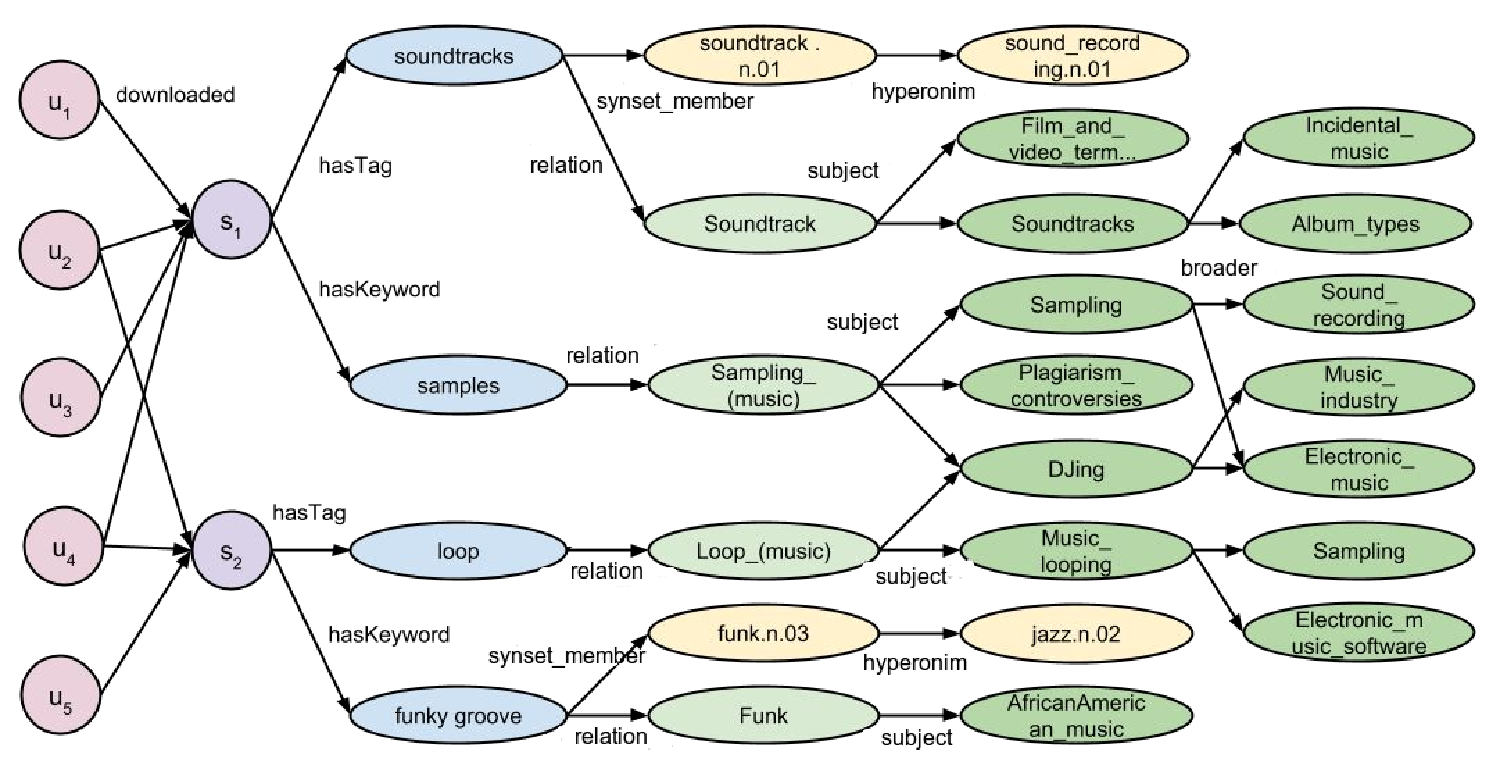
\includegraphics[width=\textwidth]{ch07_graph-rec_pics/graph_all_final2.pdf}
\caption{Portion of the final knowledge graph enriched with WordNet and DBpedia \label{fig:graph-rec:graph_enhancement}}
\end{figure*}


\section{Recommendation approach}
\label{sec:graph-rec:approach}
As aforementioned, we adopted a hybrid recommendation approach to leverage both collaborative information coming from the user's community and content information coming from the knowledge graph. 
Following the taxonomy of hybrid recommender systems presented in \cite{Burke2002} we developed a hybrid feature combination recommender system. 
The particularity of such schema is that hybridization is not based on the combination of different recommendation components but instead on the combination of different data sources. 
Specifically, collaborative information is treated as additional features of the content feature space and a content-based technique is used over this augmented space. Therefore, we build feature item representations by considering the item graph-based descriptions represented in the knowledge graph and enrich such feature vectors with collaborative features. Subsequently, we use such data to feed a content-based recommendation engine. 

A common way of computing content-based recommendation is learning a function that, for each item in the system, predicts the relevance of such item for the user. 
The application of Machine Learning techniques is a typical way to accomplish such task. % \cite{pazzani}. 
A \textit{top-N}\xspace item recommendation problem in a standard content-based setting is mainly split into two different tasks: 
(i) given a collection of items for which past user's preferences are available, learn a regression or classification model to predict the relevance associated to unknown items; (ii) eventually, according to such scores, recommend the most relevant items to the user. 
Past user's preferences can be obtained from either explicit or implicit feedback. As for Freesound, we considered as an implicit positive feedback the ``download data''. The rationale behind our choice is that if a user downloads a sound it is reasonable to assume that she likes it even without an explicit rating, as the system lets users listen to sounds before downloading. Also the Last.fm dataset used in the experimental evaluation contains user song listening actions, which is another form of implicit feedback. 
Thus, in the following we will refer to the problem of computing recommendations from implicit feedback data. 
Following the notation introduced by \cite{RendleFGS09} for implicit feedback scenarios, let $S$  be the matrix of implicit feedback, where $s_{ui}=1$ if item $i$ was downloaded from user $u$, 0 otherwise. 
Starting from $S$ we define $I_u^+ = \lbrace i \in I |  s_{ui}=1\rbrace$ as the set of relevant items for $u$. 
The main problem with implicit feedback is that they reflect only positive user preferences. On the contrary, the system cannot infer anything about what the user dislikes. The unobserved data are a mixture of actually negative and missing values \citep{RendleFGS09}, but the system does not have any information for discriminating between them. 
Then, learning a predictive model from such unary data becomes infeasible because there are no negative examples. To overcome this issue for each user we select a portion of unobserved items $I_u^- \subset (I \setminus I_u^+)$ to be used as negative data points in the training of the model. In \cite{Ostuni2013}, the authors show that choosing $|I_u^-| = 2\cdot |I_u^+|$ does not affect accuracy results.
The unobserved items are exactly the items that have to be ranked. The ultimate goal of the system is to rank in the \textit{top-N}\xspace positions items likely to be relevant for the user. 

Given the generic user $u$, let $T_u$ be the training set for $u$ defined as:
\[
T_u=\lbrace \langle x_i,s_{ui} \rangle |  i \in (I_u^+ \cup I_u^-)\rbrace
\] 
where $x_i \in \mathbb{R}^D$ is the feature vector associated to the item $i$ and let $TS_u$ be the test set defined as:
\[
TS_u=\lbrace \langle x_i,s_{ui}^* \rangle |  i \in (I \setminus I_u^+)\rbrace
\]
The two tasks for the \textit{top-N}\xspace recommendation problem, in our setting, consist then of: (i) learning a function $f_u:\mathbb{R}^D \rightarrow \mathbb{R}$ from the training data $T_u$  which assigns a relevance score to the items in $I$; (ii) using such function to predict the unknown score $s_{ui}^*$ in the test set $TS_u$, to rank them and recommend the \textit{top-N}\xspace.
%\begin{enumerate}
%\item learning a function $f_u:\mathbb{R}^D \rightarrow \mathbb{R}$ from the training data $T_u$  which assigns a relevance score to the items in $I$;
%\item using such function to predict the unknown score $s_{ui}^*$ in the test set $TS_u$, rank them and recommend the \textit{top-N}\xspace.
%\end{enumerate}

Given that items are represented as entities in a knowledge graph we are particularly interested in those machine learning methods that are appropriate for dealing with objects structured as graphs. 
There are two main ways of learning with structured objects. The first is to use \textit{Kernel Methods} \citep{Cristianini}. 
Given two input objects $i$ and $j$, defined in an input domain space $D$, the basic idea behind Kernel Methods is to construct a kernel function $k: D \times D \rightarrow \mathbb{R}$, that can be informally seen as a similarity measure between $i$ and $j$. This function must satisfy $k(i,j) = \langle \phi(i),\phi(j) \rangle$ for all $i,j \in D$, where $\phi :D \rightarrow F$ is a mapping function to a inner product feature space $F$. 
Then, the classification or regression task involves linear convex methods based exclusively on inner products computed using the kernel in the embedding feature space. 
The alternative way is to explicitly compute the \textit{explicit feature mapping} $\phi(i)$ and to directly use linear methods in the related space. 
By transforming the graph domain into a vector domain any traditional learning algorithm working on feature vectors can be applied. 

While kernel methods have been widely applied to solve different tasks, their usage becomes prohibitive when dealing with large datasets. 
%because of their scalability bottleneck. % \cite{Pham2013}. 
In addition, when the input data lie in a high-dimensional space, linear kernels have performances comparable to more complex non linear ones. 
Due to the high volume of users we deal with in our Freesound dataset (see Section \ref{sec:graph-rec:evaluation}), we focused on learning methods which are computationally efficient. For this reason we adopted the approach of computing the explicit feature mapping of the item graphs and use linear methods to learn the user model. Specifically, we use the Linear Support Vector Regression \citep{HoL12} algorithm. 
Regarding the explicit feature mapping computation we define two sparse high-dimensional feature maps: the one based on entities, the other on paths that we call \textit{entity-based item neighborhood mapping} and \textit{path-based item neighborhood mapping}, respectively. In the following we formalize the computation of such graph embeddings.

\subsection{Explicit feature mappings for graph-based Item Representations}
%Let us formally define the knowledge graph as a multi-relational graph $G=\lbrace t \mid t \in E \times R \times E \rbrace$, where $E$ denotes the set of entities and $R$ indicates the set of properties or relations, namely the edge labels. Moreover, we have $I \subseteq E$ since we consider items as a particular type of entities.\\
%With $E^h_i$ we denote the set of entities reachable in \textit{at most h} hops from $i$ according to the shortest path in $G$. For a generic item $i$ we then define its h-hop neighborhood graph $G^h_i=\lbrace t=(e_i,r_j,e_k) \mid t \in E^h_i \times R \times E^h_i \rbrace$ that is the subgraph of $G$ induced by the set of triples involving entities in $E^h_i$. 

Following the formal definition of a multi-relational knowledge graph $G=\lbrace t \mid t \in E \times R \times E \rbrace$ and an h-hop item neighborhood graph $G^h_i=\lbrace t=(e_i,r_j,e_k) \mid t \in E^h_i \times R \times E^h_i \rbrace$ stated in Section~\ref{sec:similarity:method:sim:mcs}, Figure \ref{fig:graph-rec:Example} shows an example of 2-hop item neighborhood graph for item $i$, namely $G^2_i$. We see that, if we consider the shortest path, all the entities are no more than 2 hops distant from $i$. 

\begin{figure}
\begin{center}
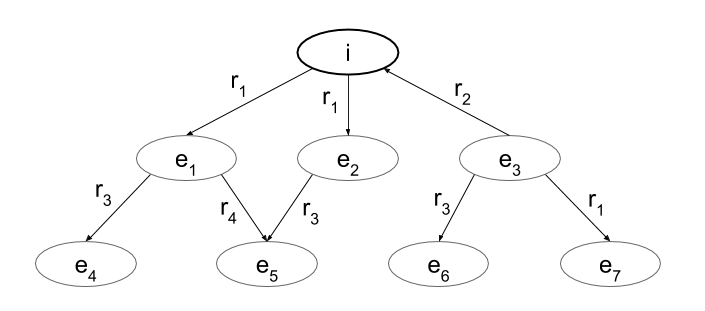
\includegraphics[width=0.8\textwidth]{ch07_graph-rec_pics/item_neig2.png}
\end{center}
\caption{An example of 3-hop item neighborhood graph for the item $i$.}
\label{fig:graph-rec:Example}
\end{figure}

To clarify the definition and computation of $G^h_i$ and $E^h_i$ for item $i$, we show their computation with reference to the example shown in Figure \ref{fig:graph-rec:Example}:\\ 
$G^1_i= \lbrace (i,r_1,e_1), (i,r_1,e_2), (e_3,r_2,i)\rbrace$\\ 
$G^2_i= G^1_i \bigcup \lbrace (e_1,r_3,e_4), (e_1,r_3,e_5), (e_2,r_4,e_5), (e_3,r_6,e_6),(e_3,r_1,e_7) \rbrace$\\
$E^1_i= \lbrace e_1, e_2, e_3 \rbrace$\\
$E^2_i=  E^1_i \bigcup  \lbrace e_4, e_5, e_6, e_7 \rbrace$\\

Starting from those item graph-based representations we define the two different feature mappings which are described in what follows.
\paragraph*{\textbf{Entity-based item neighborhood mapping}}
In this mapping each feature refers to an entity in $E$ and the corresponding score represents the weight associated to that entity in $G^h_i$. The resulting feature vector $\phi_E(G^h_i)$ is:
\[
\phi_E(G^h_i)=(w_{i,e_1} ,w_{i,e_2} ,...w_{i,e_m} ,...,w_{i,e_t} )
\]
where the weight associated to the generic entity $e_m$ is computed as follows:

\[
w_{i,e_m}=\sum \limits_{l=1}^{h} {\alpha_l \cdot c_{l,e_m}}
\] 
with 
\[
\alpha_l =\frac{1}{1+\log(l)}
\]
and
%\[
%c_{l,e_m} = \vert \lbrace  (e_n,p,e_m) \textit{  } | \textit{  } e_n \in \widehat{E}^{l-1}_i \textit{ } \vee \textit{ } e_m \in \widehat{E}^l_i \rbrace  \bigcup \]\\
%\[ \lbrace  (e_m,p,e_n) \textit{  } | \textit{  } e_m \in \widehat{E}^l_i  \textit{ } \vee \textit{ }  e_n \in \widehat{E}^{l-1}_i \rbrace \vert
%\]
\begin{multline}
c_{l,e_m} = \vert \lbrace  (e_n,r,e_m) \textit{  } | \textit{  } e_n \in \widehat{E}^{l-1}_i \textit{ } \wedge \textit{ } e_m \in \widehat{E}^l_i \rbrace 
 \bigcup \\ \lbrace  (e_m,r,e_n) \textit{  } | \textit{  } e_m \in \widehat{E}^l_i  \textit{ } \wedge \textit{ }  e_n \in \widehat{E}^{l-1}_i \rbrace \vert \nonumber
\end{multline}
where $ \widehat{E}^l_i =  E^l_i \setminus E^{l-1}_i$ is the set of entities \textit{exactly l} hops far from $i$. 
\\In particular, $c_{l,e_m}$ corresponds to the number of triples connecting $e_m$ to entities in the previous hop \textit{$(l-1)$}, whether $e_m$ appears either as subject or object of the triple. In other words, $c_{l,e_m}$ can be seen as the \textit{occurrence} of the entity $e_m$ in the item neighborhood at distance $l$. 
The more the entity $e_m$ is connected to neighboring entities of $i$, the more it is descriptive of $i$. 
$\alpha_l$ can be seen as a decay factor depending on the distance $l$ from the item $i$, whose aim is to incrementally penalize farther entities from the item. It allows us to take into account the \textit{locality} of those entities in the graph neighborhood. The closer an entity $e_m$ to the item $i$, the stronger its relatedness to it. We use a logarithmic decay. 
%Indeed, the discount factor can also be parametrized defining a specific weight for each hop. In such case, an optimal combination of weights can be found.

With reference to example showed in Figure \ref{fig:graph-rec:Example}, the $c_{l,e_m}$ values are computed as follows: 
$c_{1,e_1} =1$, $c_{1,e_2} =1$, $c_{1,e_3} = 1$, $c_{2,e_4} = 1$, $c_{2,e_5} =2$, $c_{2,e_6} =1$, $c_{2,e_7} =1$.%, $c_{2,e_8} =1$, $c_{3,e_9} =2$, $c_{3,e_{10}} =2$, $c_{3,e_{11}} =1$. All the others are zero.
%The presented graph embedding is an adaptation of the one presented in \cite{ODMD14a}, in this chapter we use a logarithmic discount factor instead of a parametric one.  

%In this mapping each feature refers to an entity in $E$ and the corresponding score represents the weight associated to that entity in $G^h_i$. The resulting feature vector $\phi_E(G^h_i)$ is:
%%\begin{small}
%\[
%\phi_E(G^h_i)=(w_{i,e_1} ,w_{i,e_2} ,...w_{i,e_m} ,...,w_{i,e_t} )
%\]
%where the weight associated to the generic entity $e_m$ is computed as follows:
%\[
%w_{i,e_m}=\sum \limits_{l=1}^{h} { \frac{ c_{l,e_m}}{1+\log(l)}} 
%\] 
%with 
%\[
%c_{l,e_m} = \vert \lbrace  (e_n,p,e_m) \textit{  } | \textit{  } e_n \in \widehat{E}^l_i \vee e_m \in \widehat{E}^l_i \rbrace \vert
%\]
%%\end{small}
%where $ \widehat{E}^l_i =  E^l_i \setminus E^{l-1}_i$ is the set of entities \textit{exactly l} hops far from $i$. 
%In particular, $c_{l,e_m}$ corresponds to the number of triples involving $e_m$, that is the \textit{occurrence} of the entity $e_m$ in the item neighborhood at distance $l$. The more the entity $e_m$ appears in paths originated by $i$, the more it is descriptive of $i$. The denominator can be seen as a decay factor depending on the distance $l$ from the item $i$, whose aim is to incrementally penalize entities farther from the item. It allows us to take into account the \textit{locality} of those entities in the graph neighborhood. The closer an entity $e_m$ to the item $i$, the stronger its relatedness to it. The presented mapping is an adaptation of the one presented in \cite{ODMD14a}.
\paragraph*{\textbf{Path-based item neighborhood mapping}}
Differently from the previous case, in this mapping we represent a feature as a sequence of nodes in $G$. Given two entities $e_1$ and $e_n$, we consider the sequence of nodes $e_1 \cdot e_2 \cdot \ldots \cdot e_{n-1} \cdot e_n$ met while traversing the graph to go from $e_1$ to $e_n$ and we refer to such sequence as \textit{path}. In this  mapping, a feature is then represented by a path. In particular, in this mapping each feature refers to several variants of paths rooted in the item node. 
We first collect all the paths rooted in $i$ which can be indicated as sequence of entities $i\cdot e_1 \cdot e_2 \cdot \ldots \cdot e_{n-1} \cdot e_n$. 
Then, starting from those paths we define various features considering sub-paths of the original paths. Specifically we form sub-paths composed by only those entities progressively farther from the item.
Considering the path given above we build the following features: $e_1 \cdot e_2 \cdot  \ldots \cdot  e_{n-1} \cdot  e_n$, $e_2 \cdot  \ldots \cdot  e_{n-1} \cdot  e_n$, ..., $e_{n-1} \cdot  e_n$, $e_n$. 
The rationale behind this choice is that it allows to explicitly represent substructures shared between items with no overlapping in their immediate neighborhoods but somehow connected at further distance. Items connected to the same entities have same common structures because both closer and further entities are shared. Items connected to different entities which are however linked directly or at a farther distance to same entities  share less or none sub-paths depending on how much far the common entities are, if any.

More formally, let $P_i$ be the set of paths rooted in $i$ and $P^*_i$ be the list of all possible sub-paths extracted from them. We use $p_m(i)$ and $p^*_m(i)$ to refer to the $m-th$ elements in $P_i$ and $P^*_i$, respectively. Then, the feature mapping for item $i$ is:
\[
\phi_P(G^h_i)=(w_{i,p^*_1} ,w_{i,p^*_2} ,...w_{i,p^*_m} ,...,w_{i,p^*_t} )
\]
% paths making up part of larger paths. 
where each $w_{i,p^*_m}$% is the frequency of the feature $p_m$ in $G^h(i)$.  
is computed as:
\[
w_{i,p^*_m}=  \frac{ \# p^*_m(i) }{ \vert p_m \vert - \vert p^*_m \vert} 
\] 
where $\vert p_m \vert$ indicates the length of path $p_m$ and $\# p^*_m(i)$ the occurrence of $p^*_m(i)$ in $P^*_i$. The denominator is a discounting factor which takes into account the difference between the original path $p_m$ and its sub-path $p^*_m$. The shorter the sub-path the more the discount because it contains entities farther from the item. 
\\With respect to item $i$ we have:\\
$P_i= \lbrace i \cdot e_1 \cdot e_4,\text{ }i \cdot e_1 \cdot e_5,\text{ } i \cdot e_2 \cdot e_5,\text{ } i \cdot e_3 \cdot e_6,\text{ } i \cdot e_3 \cdot e_7 \rbrace$\\
$P^*_i= [ e_1 \cdot e_4,\text{ } e_4,\text{ } e_1 \cdot e_5,\text{ }e_5,\text{ } e_3 \cdot e_6,\text{ } e_6
,\text{ } e_3 \cdot e_7,\text{ } e_7 ]$

%Differently from the previous mapping, in this mapping features are represented as a sequences of nodes in $G$. Given two entities $e_1$ and $e_n$, we consider the sequence of nodes $e_1 \cdot e_2 \cdot \ldots \cdot e_{n-1} \cdot e_n$ met while traversing the graph to go from $e_1$ to $e_n$ and we refer to such sequence as \textit{path}. In this  mapping, a feature is then represented by a path. In particular, in this mapping each feature refers to several variants of paths rooted in the item node.
%We first collect all the paths rooted in $i$ which can be indicated as sequence of entities $i\cdot e_1 \cdot e_2 \cdot \ldots \cdot e_{n-1} \cdot e_n$. 
%Then, starting from those paths we define various features considering sub-paths of the original paths. Specifically we form sub-paths composed by only those entities progressively farther from the item.
%Considering the path given above we build the following $n$ features: $e_1 \cdot e_2 \cdot  \ldots \cdot  e_{n-1} \cdot  e_n$, $e_2 \cdot  \ldots \cdot  e_{n-1} \cdot  e_n$, ..., $e_{n-1} \cdot  e_n$, $e_n$. 
%The rationale behind this choice is that it allows to explicitly represent substructures shared between items with no overlapping in their immediate neighboorhoods but somehow connected at further distance. Items connected to the same entities have same common structures because both closer and further entities are shared. Items connected to different entities which are however linked directly or at a farther distance to same entities  share less or none sub-paths depending on how much far the common entities are, if any.
%
%More formally, let $P_i$ be the set of paths rooted in $i$ and $P^*_i$ all possible sub-paths extracted from them. We use $p_m(i)$ and $p^*_m(i)$ to refer to the $m$-th elements in $P_i$ and $P^*_i$, respectively. Then, the feature mapping for item $i$ is:
%\[
%\phi_P(G^h_i)=(w_{i,p^*_1} ,w_{i,p^*_2} ,...w_{i,p^*_m} ,...,w_{i,p^*_t} )
%\]
%% paths making up part of larger paths. 
%where each $w_{i,p^*_m}$% is the frequency of the feature $p_m$ in $G^h(i)$.  
%is computed as:
%\[
%w_{i,p^*_m}=  \frac{ \# p^*_m(i) }{ \vert p_m \vert - \vert p^*_m \vert} 
%\] 
%Here $\vert p_m \vert$ indicates the length of path $p_m$ and $\# p^*_m(i)$ the occurrence of $p^*_m(i)$ in $P^*_i$. The denominator is a discounting factor which takes into account the difference between the original path $p_m$ and its sub-path $p^*_m$. The shorter the sub-path the more the discount because it contains entities farther from the item. 
\subsection{Feature Combination}
Each final feature vector $x_i$ is obtained by concatenating a vector of collaborative features $\phi_{col}(i)$ to the item neighborhood mapping vector $\phi(G^h_i)$. Collaborative features are simply added by encoding in the feature vector those users who downloaded that item. The collaborative feature vector regarding the generic item is then:
\[
\phi_{col}(i)=(w_{i,u_1}, w_{i,u_2},...,w_{i,u_1})
\]
where $w_{i,u_1}=1$ if user $u_1$ downloaded item $i$.

Although more sophisticated and advanced methods can be used for feature combination \citep{Beliakov2015}, our experimental evaluation (see Section \ref{sec:graph-rec:evaluation}) shows the effectiveness of our choice.   
%\subsection{Audio-based approach}
%For evaluation purposes, we created a recommendation approach based only on audio content features. Apart from text descriptions and tags, Freesound provides information about acoustic features of the sound signal. Every sound in Freesound is analyzed at the time of the upload using Essentia~\citep{Bogdanov2013}, a library for audio analysis. Moreover, a distance measure between sounds is provided and sounds can be retrieved according to this measure. To calculate the distance between sounds, Personal Component Analysis (PCA) is applied over 352 low-level audio descriptors, reducing the space to 100 dimensions. Then, the euclidean distance between sounds is calculated over the reduced space. 
%
%We define the similarity between two sounds $s_1$, $s_2$ as $sim(s_1,s_2)=1-dist(s_1,s_2)$, being $dist(s_1,s_2)$ the normalized value of the euclidean distance. Based on this measure, we created a simple content-based recommender system. For every user, we ranked all sounds $s_i \in TS_u$ by computing the formula 
%\[
%Score(u,s_i) = \frac{\sum \limits_{ j\in I_u^+}{sim(s_i,s_j)}}{|I_u^+|}
%\]




\section{Experimental Evaluation}
\label{sec:graph-rec:evaluation}
For the evaluation of our approach we adopted the \texttt{All Unrated Items} methodology presented in \cite{Steck13}. It consists in creating a \textit{top-N}\xspace recommendation list for each user by predicting a score for every item not rated by that particular user, whether the item appears in the user test set or not. Then, performance metrics are computed comparing recommendation lists with test data.  
The evaluation has been carried out using the holdout method consisting in splitting the data in two disjoint sets: the one for training and the other for testing. We used 80\% of user downloads for building the training set $T$ and remaining 20\% as test data for measuring recommendation accuracy. We repeated the procedure three times by randomly drawing new training/test sets in each round and averaged the results.
%The tuning of model hyper-parameters of the learning algorithm was performed through cross-validation on validation data obtained by selecting the 15\% of feedback for each user from the training data. Specifically we adopted the \textit{LIBLINEAR\footnote{\url{http://www.csie.ntu.edu.tw/~cjlin/liblinear/}}} library. We used the \textit{L2-regularized Support Vector Regression} \cite{HoL12} method and chose the $C$ and $e$ parameters via cross-validation using a grid-search varying $C$ from 0.1 to 1000 with step 10 and $e=\lbrace 0.1,0.01 \rbrace$ (tolerance of termination criterion). Before the training we performed some pre-processing on the feature vectors. We removed those features appearing in less then 5  sounds and scaled all features to the range $[0-1]$ using min-max normalization. Finally each feature vector was normalized to unit length using the L2 norm.

%\subsection{Evaluation Metrics}
For measuring recommendation accuracy we adopted the following standard performance metrics: Precision and Recall. 
Precision@N (P@N) is computed as the fraction of \textit{top-N}\xspace recommended items appearing in the test set, while Recall@N (R@N) is computed as the ratio of \textit{top-N}\xspace recommended items appearing in the test set to the number of items in the test set. Note that in such implicit feedback setting all items in the test set are relevant. In addition to the standard precision and recall metrics we also measure the Mean Reciprocal Rank (MRR) which measure the quality of the highest ranked recommendations. For each user recommendation list the Reciprocal Rank (RR) measures how early in the list is positioned the first relevant recommendation. 

As pointed out by \cite{McNee2006}, the most accurate recommendations according to the standard metrics are sometimes not the recommendations that are most useful to users. In order to assess the utility of a recommender system, it is extremely important to evaluate also its capacity to suggest items that users would not readily discover for themselves, that is its ability to generate novel and unexpected results.
The \textit{Entropy-Based Novelty} (\textit{EBN}) \citep{Bellogin2010} expresses the ability of a recommender system to suggest less popular items, i.e. items not known by a wide number of users. 
In particular, for each user's recommendation list $L_u$, the novelty is computed as:  
\[ EBN_u@N = - \sum \limits_{ i\in L_u} p_i \cdot \log_{2} p_i \]
where:
\[    p_i = \frac{ \vert \lbrace s_{ui}=1 \vert u \in U \rbrace \vert}{  \vert  U  \vert } \]
\noindent Particularly, $p_i$ is the ratio of users who downloaded item \textit{i}. The lower $EBN_u@N$, the better the novelty.

Another important quality of the system is aggregate diversity. 
%its level of personalization which can be measured looking at the aggregate diversity of recommendations across all users. 
In our chapter we adopt the \textit{diversity-in-top-N} metric presented in \cite{AdomaviciusK12} that measures the distinct items recommended across all users. In particular we compute its normalized version with respect to the size of the item catalog. For brevity we refer to it as $ADiv@N$ and we compute it as follows:
\[ ADiv@N = \frac{ \vert \bigcup_u L_u \vert }{ \vert I \vert }  \]
This metric is an indicator of the level of personalization provided by a recommender system. Low values of aggregated diversity indicate  that all users are being recommended almost the same few items. This corresponds to a low level of personalization of the system. Instead, high values mean that users receive very different recommendations which can be indirectly seen as a high level of personalization of the system. %The importance of such particular dimension of the recommendation quality has been also highlighted in other chapters as in \cite{JannachLGB13}.

All the reported metrics, besides aggregated diversity, are computed for each single user and eventually averaged.

\subsection{Datasets Description}
\label{sec:graph-rec:datasets}

\paragraph*{\textbf{Freesound Dataset}}\label{fs_dataset}
We evaluated our approach on historical data about sound downloads collected from February 2005 to October 2013. In addition, we further enriched our knowledge graphs (see Section~\ref{sec:graph-rec:enrichment}) with information coming from the Freesound Ontology \citep[chapter 6]{font2015tag}, a lightweight ontology where the 500 most popular Freesound tags are classified into 23 tag categories. From the original data dump, we selected a subset of sounds that fulfilled some criteria. We selected those sound with at least two tags classified in the Freesound Ontology. After that we filtered out all sounds with less than 10 downloads to reduce the sparsity of the implicit feedback matrix and have a fairer comparison with pure collaborative filtering methods. 
%After this initial filtering, a total number of 99,008 sounds were obtained out of which 22,000 were randomly selected. Among them, we selected those with at least one entity detected in textual description and linked to WordNet or DBpedia and finally obtained 21,552 sounds. 
%The number of registered users that had downloaded at least 50 of these sounds was 112,723 out of which 20,000 were randomly selected. 
After some further data cleansing, the final dataset consisted in 20,000 users, 21,552 items and 2,117,698 downloads.%\footnote{A dump of the datasets is available at \url{http://mtg.upf.edu/download/datasets/knowledge-graph-rec}}. 
The sparsity of the implicit feedback matrix was 99.51\%. Statistics on the enriched knowledge graph of the final dataset are shown in Table~\ref{tbl:graph-rec:datasets}.

%The total number of different tags found in the final set of sounds was 15,096. From this tag space, 8,160 were mapped to WordNet concepts, 7,099 to DBpedia entities, and 387 were classified in the Freesound Ontology. The average number of mapped tags per item was 6.44. From the textual descriptions, a total number of 23,481 keywords were mapped to 16,706 WordNet synsets, and 16,854 DBpedia entities. The average number of mapped keywords per item was 11.36.
%{\color{red}The full dataset, including hypernyms and broader categories, contains 16,407 DBpedia entities, 54,419 Wikipedia categories, and 20,034 WordNet synsets.}
%In the whole dataset, the number of different DBpedia entities mapped to words was 16,407, and those entities were related to 35,706 different categories. Taking into account also categories connected via the \texttt{skos:broader} property, the total number of categories in the dataset was 54,419. The number of different Wordnet synsets mapped to words was 17,926, and the total number of synsets in the dataset including hypernyms was 20,034.

\begin{table}
\scriptsize
	%[!htb]
	%\tbl{Datasets Overview\label{tbl:graph-rec:datasets}}{%
%	\scriptsize
	\label{tbl:graph-rec:datasets}
	\begin{tabular}{l c c c c c c}
		\toprule
		\textbf{dataset} & \textbf{items} & \textbf{avg. tags} & \textbf{avg. keywords} & \textbf{resources} & \textbf{synsets} & \textbf{categories}\\
		\midrule
		Freesound & 21,552 & 6.44 & 11.36 & 16,407 & 20,034 & 54,419 \\
		Last.fm & 8,640 & 42.09 & 77.33 & 46,109 & 27,708 & 96,942 \\
		\bottomrule
		
	\end{tabular}
	\caption[Number of tags and keywords.]{Number of tags and keywords identified by Babelfy averaged by item, plus total number of distinct DBpedia resources, WordNet synsets and Wikipedia categories.
	}
\end{table}


\paragraph*{\textbf{Last.fm Dataset}}\label{fs_dataset}
To recreate most of the conditions of the Freesound dataset in a music recommendation scenario, a new dataset is created combining user's implicit feedback, tags and textual descriptions of songs. This dataset combines a corpus of user's listening habits \citep{Vigliensoni2014}, with tags and textual descriptions about songs. For every user in the corpus we chose the users' average listening count as a threshold to identify the relevant songs for each user. We only selected for our implicit feedback dataset user-song relations with a number of listens above each user's threshold. Moreover, only those songs that were relevant to at least 10 users, and users with at least 50 relevant songs were added to the dataset. The final dataset consisted in 5,199 users, 8,640 songs and 751,531 relations between users and songs. The sparsity of the implicit feedback matrix was 98.33\%.
This collaborative information was complemented with the list of top tags of every song provided by the Last.fm API, and a textual description of each song coming from Songfacts.com (cf. Section~\ref{sec:kb:exp:dataset}). Information about the enriched knowledge graph is shown in Table~\ref{tbl:graph-rec:datasets}.
%We applied the same semantic enrichment process described in Section~\ref{sec:enrichment} to tags and text descriptions. A total number of 38,796 DBpedia entities, 88,556 Wikipedia categories and 15,995 WordNet synsets were added to the Knowledge Graph. The average number of mapped keywords per item was 99.6.


\subsection{Experiment settings}
As mentioned in Section \ref{sec:graph-rec:approach}, each user model is learnt using the Linear Support Vector Regression method. In particular we adopted the efficient \textit{LIBLINEAR\footnote{\url{http://www.csie.ntu.edu.tw/~cjlin/liblinear/}}} library and chose the \textit{L2-regularized Support Vector Regression} \citep{HoL12}. 
The tuning of the model hyper-parameters of the learning algorithm was performed through cross-validation on validation data obtained by selecting the 15\% of feedback for each user from the training data. We set the parameters $C$ and $e$ by using a grid-search varying $C$ from 0.1 to 1000 with step 10 and $e=\lbrace 0.1,0.01 \rbrace$ (tolerance of termination criterion). Before the training we performed some pre-processing on the feature vectors. We removed those features appearing in less than 5 items and scaled all features to the range $[0,\ldots,1]$ using min-max normalization. Finally each feature vector was normalized to unit length using the L2 norm.

%Regarding the run time performances of the entire recommender for the Freesound experiment, the highest computation time (corresponding to the path-based feature mapping with 3-hops) lasted about 28 minutes, from feature extraction to recommendation generation, on a dedicated server machine with 4 Xeon quad-core 2.93GHz processors and 32GB RAM. 
%Since each user model is learnt independently, the learning process is highly parallelizable.  Moreover, being a model-based recommender, each user model learning can be performed offline periodically once a certain number of new feedbacks are accumulated for that specific user. 
%The implementation of the recommendation algorithm presented in this chapter is available on GitHub \footnote{\url{https://github.com/sisinflab/lodreclib}}.

In the following we describe the experiments we carried out to evaluate our approach. In particular we are interested in evaluating the impact of semantic enrichment of the original data on the recommendation quality and the differences among the two feature mapping methods we implemented. Furthermore, we compare our approach with state of the art algorithms for implicit feedback scenarios. 
All the differences between approaches and with respect to other baselines are statistically significant ($p<0.01$) according to the paired t-test.


%%%%%%%%%%%%%%%%%%%%%%%%%%%%%%%%%%%%%%%%%%%%%%%%%%%%%%%%%%%%%%%%%%%%%%%%%%%%%%%%%%%%
\begin{table}
\scriptsize
	%[!htb]
	%\tbl{Freesound Results\label{tbl:graph-rec:Res1}}{%
%	\scriptsize
	\label{tbl:graph-rec:Res1}
\begin{tabular}{l l c c c c c c }
		\toprule
		\textbf{Approach} & \textbf{Enrichment} & \textbf{h-hops} & \textbf{MRR} &  \textbf{P@10} & \textbf{R@10} & \textbf{EBN@10}  & \textbf{ADiv@10}\\
		\midrule
		Ent & fso & h=3 & 0.303 & 0.113  &  0.065 & 2.791	& 0.257   \\
		Ent & fso+KB/tag & h=3 & 0.303 & 0.115  &  0.066  & 2.617 &	0.332  \\
		Ent & fso+KB/tag & h=4 & 0.302 & 0.114  & 0.065  & 2.507 & 0.368  \\
		Ent & fso+KB/kw+tag & h=3 & \textbf{0.306 }& \textbf{0.118}  &  \textbf{0.067}  & 2.426 &	0.361  \\
		Ent & fso+KB/kw+tag & h=4 & \textbf{0.306}  & 0.117 & 0.066  &2.303  & 0.391   \\ 
		Path & fso & h=3 &  0.301 &  0.113  &  0.065   & 2.750 & 0.287   \\
		Path & fso+KB/tag & h=3 & 0.301 &  0.114 &  0.064 & 2.279 	& 0.461   \\
		Path & fso+KB/tag & h=4 &   0.292 & 0.106 & 0.059   & 1.863 & \textbf{0.556*}   \\
		Path & fso+KB/kw+tag & h=3 &  0.304 & 0.116 &  0.065    & 2.019 &	0.461     \\
		Path & fso+KB/kw+tag & h=4 & 0.296 & 0.111 &	0.061      & \textbf{1.618*}	& 0.532   \\
		\midrule
		Col & & & 0.293 & 0.110 & 0.062 &	2.890 &	0.181 \\	
		Ent-noCol & fso+KB/kw+tag & h=3 & 0.154   & 0.058	 &0.034	  & 0.384	& 0.591   \\		
		Path-noCol & fso+KB/kw+tag & h=3 & 0.151 & 0.049 & 0.028  & \textbf{0.369} & \textbf{0.670}   \\			
		VSM & kw+tag & h=1 & 0.301 &   0.116 &  0.066  & 2.621 &	0.305 \\
		VSM-noCol & kw+tag & h=1 & 0.151  & 0.055 	 & 0.032	& 0.389 & \textbf{0.670} \\
		Audio Sim & & & 0.022 & 0.004 & 0.002 &	0.382	&	0.044 \\
		\bottomrule
	\end{tabular}
	
	\caption[Accuracy, Novelty and Aggregate Diversity results for different versions of the Freesound dataset.]{Accuracy, Novelty and Aggregate Diversity results for different versions of the Freesound dataset. Best values in each column are in bold. The * symbol indicates best values for hybrid and collaborative configurations. \texttt{Ent} and \texttt{Path} refers to graph embedding options; \texttt{fso} to the initial Freesound Ontology, \texttt{KB} to WordNet and DBpedia enrichment; \texttt{tag} to item tags, and \texttt{kw} to text description keywords; \texttt{h} indicates the length of the h-hop neighborhood graph; \texttt{Col} means that only collaborative features are considered; \texttt{noCol} that no collaborative features are considered; \texttt{VSM} refers to Vector Space Model embedding; \texttt{Audio Sim}  to the audio-based approach.
	}
\end{table}
%%%%%%%%%%%%%%%%%%%%%%%%%%%%%%%%%%%%%%%%%%%%%%%%%%%%%%%%%%%%%%%%%%%%%%%%%%%%%%%%%%%%

\subsection{Sound Recommendation Experiment}
\paragraph*{\textbf{Evaluation of the semantic item description enhancement}}\label{sem_eval}
To evaluate the impact of the various features and information sources we built several variants of item feature vectors by varying: the information sources considered, the size of the item neighborhood graphs (number of hops) and the feature mapping method. 
%The prefixes \texttt{Ent} and \texttt{Path} refer the usage of \textit{entity-based item neighborhood mapping} and \textit{path-based item neighborhood mapping} respectively.
%In \texttt{(fso)} the item neighborhood graph is built considering only the Freesound Ontology starting from the tags mapped to the ontology.  
%In \texttt{(fso+KB/h=x)} the item is represented by the corresponding \texttt{x}-hop neighborhood extracted from the FSO ontology enriched with WordNet and DBpedia. 
%Differently from \texttt{(fso+KB/h=x)}, in the configuration \texttt{(fso+KB+kw+tag/h=x)} also text descriptions are mapped to the ontology. 
%Differently from the previous cases, \texttt{VSM kw+tag} is a pure textual approach where the Vector Space Model was applied on raw tags and keywords. 
%\texttt{noCol} means that no collaborative features are considered (pure content-based approach) and \texttt{Collab} means that only collaborative features are considered (each feature vector consists of $\phi_{col}$ only). 
In addition, we built a content-based approach purely based on 352 low-level audio features\footnote{\url{https://www.freesound.org/docs/api/analysis_example.html\#all-descriptors}} extracted from the sound signal by using Essentia~\citep{Bogdanov2013}. In this approach, predictions are computed by aggregating the Euclidean distances between the sounds downloaded by the user and the target sound to recommend. %Final recommendation lists are generated by taking the sounds with lowest score.
All the results are reported in Table \ref{tbl:graph-rec:Res1}. 

Looking at the accuracy results we see that there are no marked differences among all the feature vector variants. Noteworthy is that without considering the collaborative information (\texttt{noCol}) the accuracy drops significantly. In addition, when considering only collaborative features accuracy performances are comparable with respect to hybrid feature combination variants. The best hybrid semantic version \texttt{Ent(fso+KB/kw+tag/h=3)} is slightly better than pure collaborative.% (+0.8\% in terms of P@10). 
Regarding the comparison of the two mapping methods, the Entity-based item neighborhood mapping has generally slightly higher accuracy than the Path-based one. We can also note that considering too far entities in the graph does not improve accuracy. In fact, in both the two feature mapping when four hops are considered the results drop slightly with respect to three hops. 
Finally, we see that the semantic expansion of tags and terms do not improve consistently accuracy with respect to the usage of pure keywords and tags combined with collaborative information. The semantic configuration with highest accuracy (\texttt{Ent(fso+KB/kw+tag/h=3)}) is slightly better in terms of P@10 with respect to  \texttt{VSM kw+tag}. We can also observe that the pure audio based approach (\texttt{Audio Sim}) has by far lower performances than all the others. %All the differences between the hybrid graph embeddings and the other baselines are statistically significant ($p<0.01$) according to the paired t-test.
%\\To summarize, regarding recommendation accuracy the introduction of semantics slightly increase the performances with respect to the usage of pure collaborative features and in particular when the Entity-based feature mapping is used. While collaborative features also are able to guarantee good performances, content-based features alone are not able to give such accurate recommendations. 

Novelty and aggregate diversity results instead show more interesting insights. We observe that the semantic expansion, with both feature mappings, results in an improving of both novelty and aggregated diversity. In fact, the semantic enriched variant \texttt{(fso+KB+kw+tag/h=4)} has much better novelty and diversity than considering only the original Freesound Ontology \texttt{(fso)}. Furthermore, with respect to the variants without semantic expansion, that is the variants based only on keywords and tags, the usage of semantic expansion improves considerably novelty and diversity. Hence, thanks to this exploitation of the knowledge graph we are able to recommend good items which are also not so popular. We also see that the Path-based embedding has better performances than the Entity-based one. 
Such approaches allow to explore better the long tail distribution of items and to increase the personalization of the system. 
\\The variants without collaborative information are the ones with better novelty and diversity. The reason behind this behavior is that pure content-based approaches are not influenced by popularity biases. However, when using only content data the system recommends unpopular but very inaccurate items. Good novelty without accuracy does not imply good recommendation quality. 
Finally, the usage of only collaborative information has much lower catalog coverage (aggregate diversity) than feature vectors containing also semantic features. For example \texttt{Path(fso+KB+kw+tag/h=4)} has comparable performances in terms of accuracy with respect to \texttt{Collab} but considerably better catalog coverage and novelty (lower EBN). 

To conclude, we can state that the semantic expansion, especially when combined with the Path-based mapping, improves recommendation quality in terms of novelty and aggregated diversity. The intuition behind these results is that the semantic expansion allows the system to find items semantically related to the ones in the user profile. Conversely, when using only keyword or tag-based representations the system is able to retrieve only those few items with an exact keyword/tag match with those liked by the user. Thus, the system is unable to widely explore the item space to find those items which are semantically related to the ones liked by the user.
%\vcoinline{seems that by adding data we are able to increase diversity. Is just a matter of increasing the features to diversify the feature space or adding meaningful features to increase the semantic matching among items? In the keyword approach there are few items that are similar to the ones rated by the user. this imply that the system recommends always a few items with commonalities with the user profile. With the semantic expansion, instead the items are better described and the system is able to find more items semantically similar to the user profile.}
%\vcoinline{we able to give novelty similar to cf methods. with semantics we can give better novelty than pure keyword based with comparable accuracies. the only content based gives high novelty but very poor recommendation quality. it recommends too obscure items.}
%\vcoinline{fare exp con babelfy 3 hops}
\paragraph*{\textbf{Comparison with other methods}}\label{comp}
%%%%%%%%%%%%%%%%%%%%%%%%%%%%%%%%%%%%%%%%%%%%%%%%%%%%%%%%%%%%%%%%%%%%%%%%%%%%%%%%%%%%%
\begin{figure*}
	\centering
	\begin{subfigure}[b]{\textwidth}
		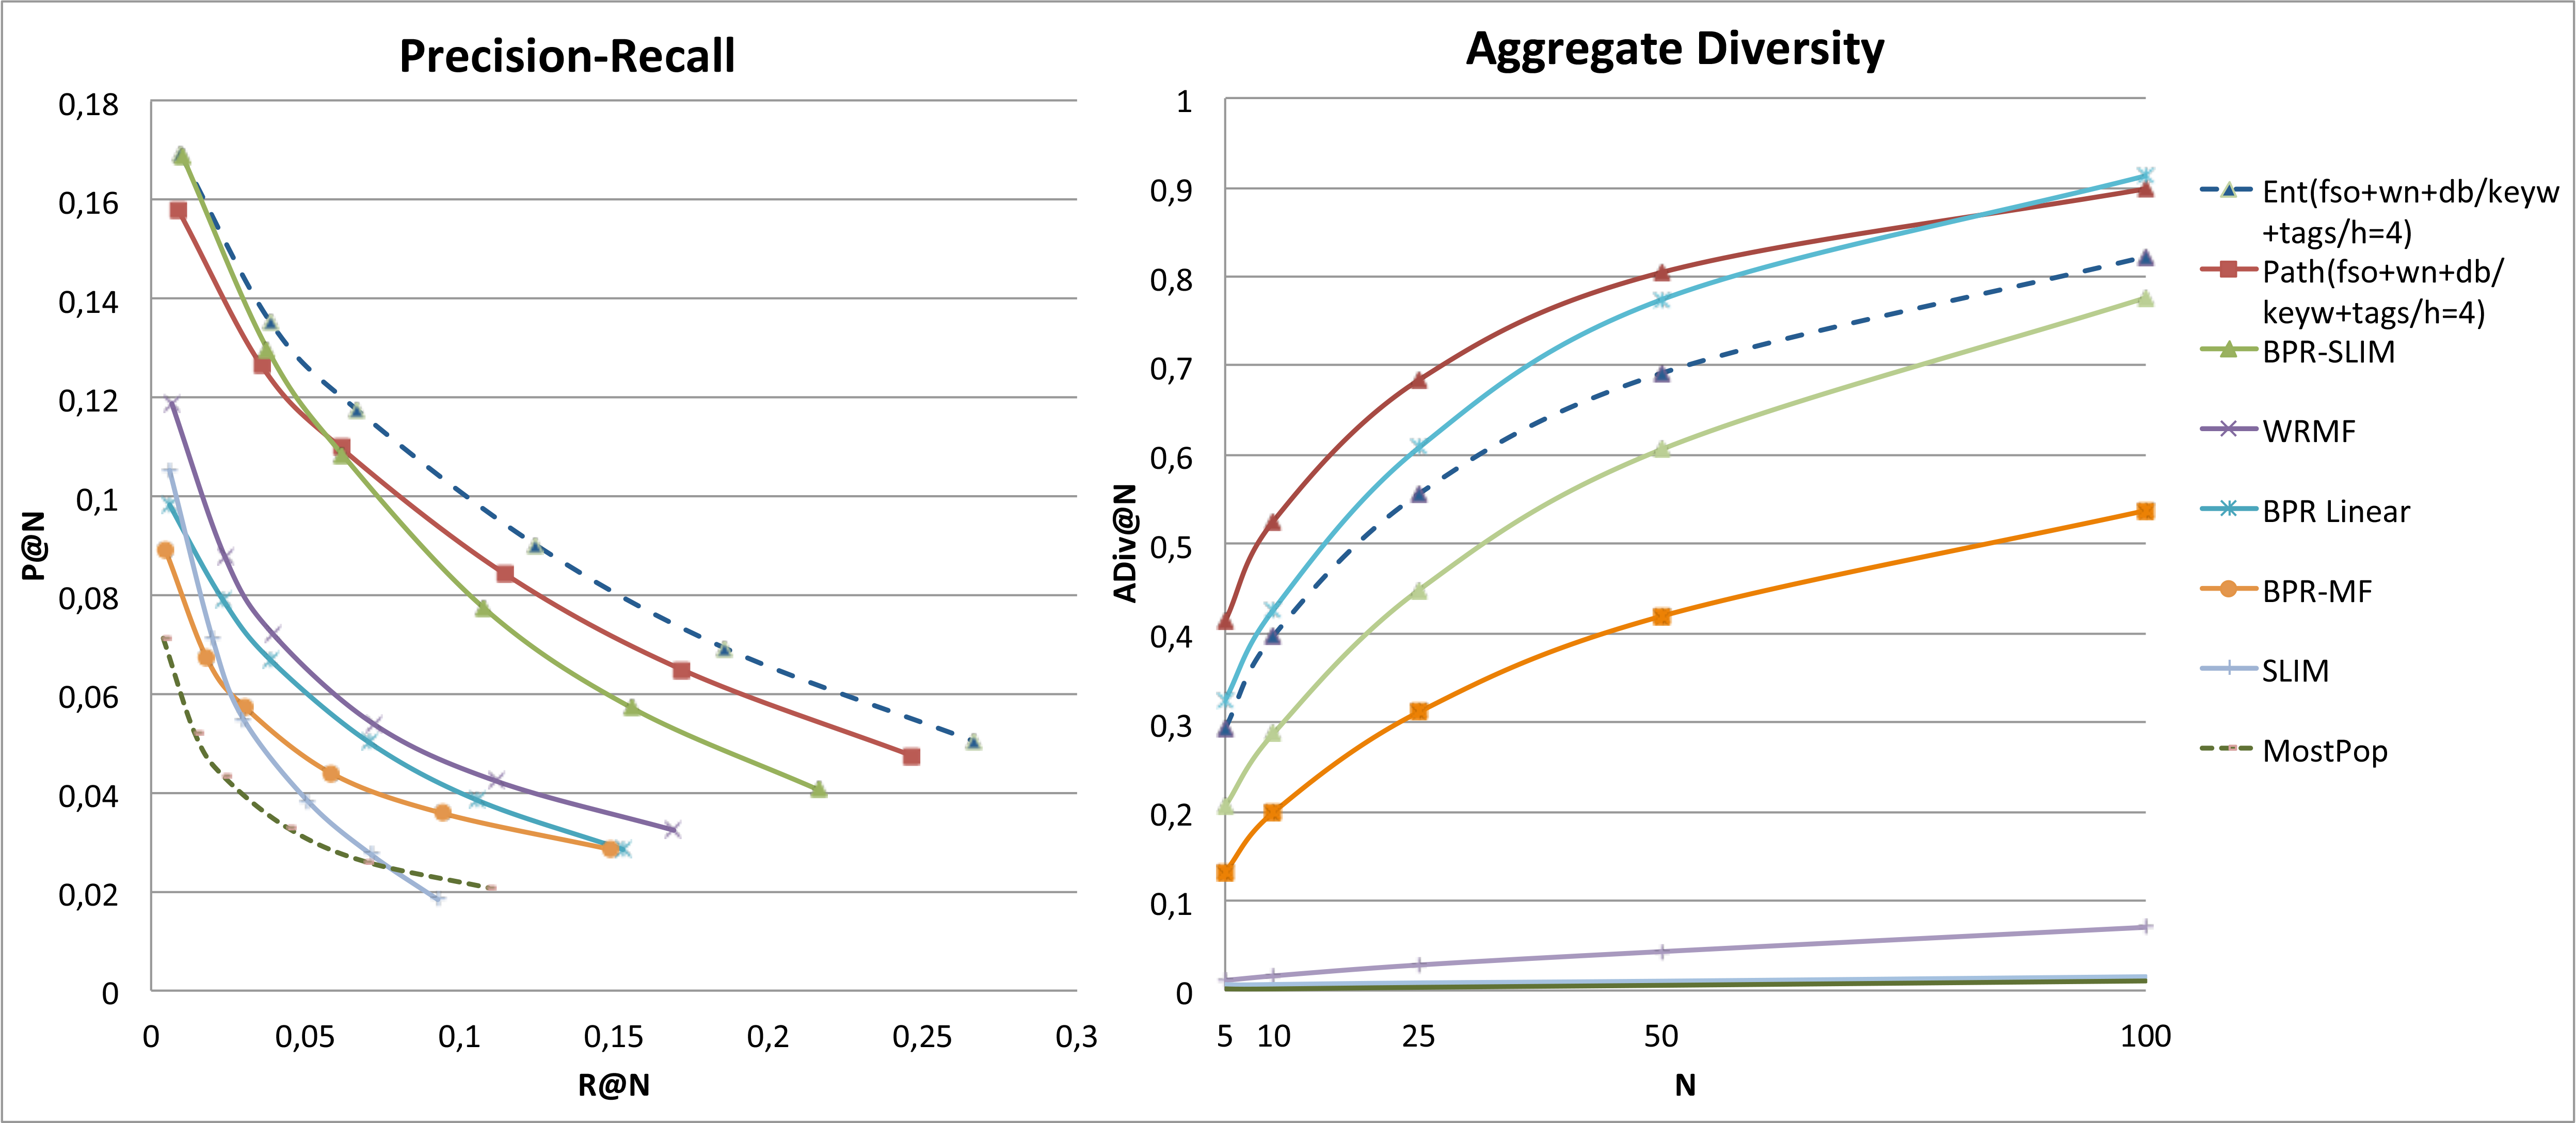
\includegraphics[width=\textwidth]{ch07_graph-rec_pics/pr_adiv_fr.png}
	\end{subfigure}
	\begin{subfigure}[b]{\textwidth}
		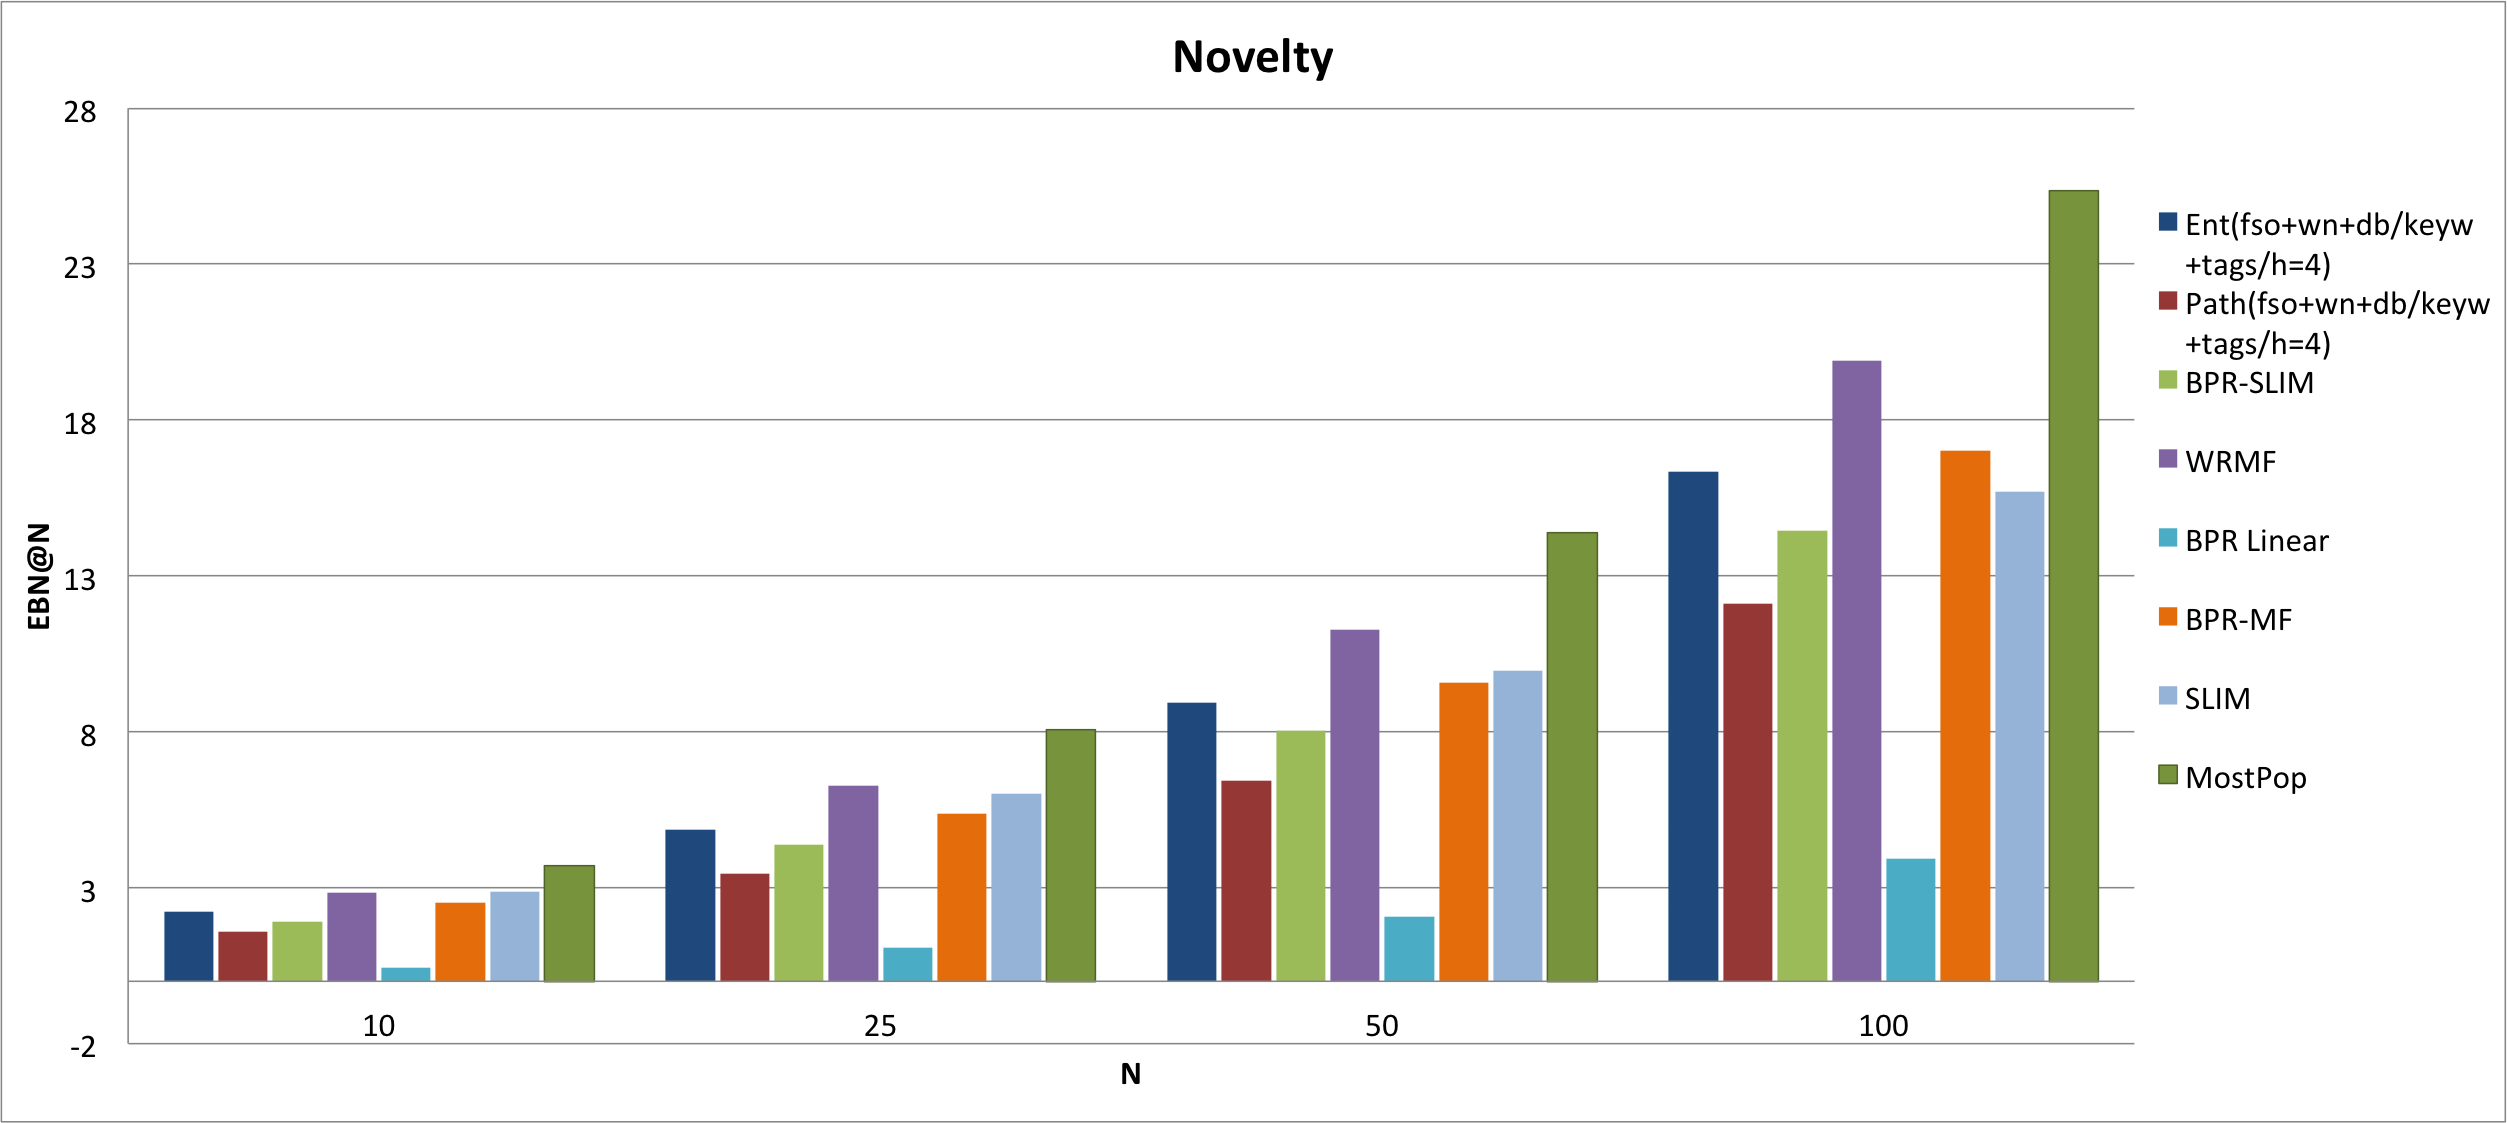
\includegraphics[width=\textwidth]{ch07_graph-rec_pics/nov_fr.png}
	\end{subfigure}
	\caption{Precision-Recall, Novelty and Aggregate Diversity plots in Freesound dataset\label{fig:graph-rec:accur}}
\end{figure*}
%%%%%%%%%%%%%%%%%%%%%%%%%%%%%%%%%%%%%%%%%%%%%%%%%%%%%%%%%%%%%%%%%%%%%%%%%%%%%%%%%%%%%
%%%%%%%%%%%%%%%%%%%%%%%%%%%%%%%%%%%%%%%%%%%%%%%%%%%%%%%%%%%%%%%%%%%%%%%%%%%%%%%%%%%%%
%\begin{figure*}
%	\centering
%	\subfigure{\includegraphics[width=1\textwidth]{ch07_graph-rec_pics/prec_rec.png}}
%	\subfigure{\includegraphics[width=1\textwidth]{ch07_graph-rec_pics/nov.png}}
%	\subfigure{\includegraphics[width=1\textwidth]{ch07_graph-rec_pics/adiv.png}}
%	\caption{Precision-Recall, Novelty and Aggregate Diversity plots\label{fig:graph-rec:accur}}
%\end{figure*}
%%%%%%%%%%%%%%%%%%%%%%%%%%%%%%%%%%%%%%%%%%%%%%%%%%%%%%%%%%%%%%%%%%%%%%%%%%%%%%%%%%%%%%
%In order to evaluate the effectiveness in terms of ranking accuracy of \framechapter we compared it with several state of the art recommendation algorithms:
%\vcoinline{cf focus too much on popular items, instead our approach is able to explore long tail items.}
We compared our approach with several state of the art recommendation algorithms. 
%\begin{scriptsize}
%\begin{itemize}
\texttt{MostPop} is a popularity-based baseline which provides the same recommendation to all users based on the global popularity of items. 
\texttt{BPR-MF} \citep{RendleFGS09} is a matrix factorization-based method optimized with Bayesian Personalized Ranking optimization criterion.
\texttt{WRMF} is a weighted matrix factorization method \citep{Hu2008}.
\texttt{SLIM} \citep{Ning2012} uses a Sparse Linear method for learning a sparse aggregation coefficient matrix.
\texttt{BPR-SLIM} is similar to \texttt{SLIM} but it uses the BPR optimization criterion.
\texttt{BPR Linear} is a hybrid matrix factorization method able to chapter with sparse datasets \citep{GantnerDFRS10}. We used keywords and tags as item attribute data. 
The computation of the recommendations for all these comparative algorithms has been done with the publicly available software library \textit{MyMediaLite}\footnote{\url{http://www.mymedialite.net/}.}.
%\citep{Gantner2011MyMediaLite}

Figure \ref{fig:graph-rec:accur} shows precision-recall, novelty and aggregated diversity plots. In those plots we report the competitive algorithms used for comparison and the \texttt{Ent(fso+KB/kw+tag/h=4)} and \texttt{Path(fso+KB+kw+tag/h=4)} configurations which we chose as representative for our approach due to its performances in terms of novelty and aggregate diversity. 
\\With reference to the accuracy results we notice that our two approaches largely outperforms the others. The only method which is close to the approaches we propose is \texttt{BPR-SLIM} which slightly outperforms \texttt{Path(fso+KB+kw+tag/h=4)} for low values of recommendation list length ($N=5,10$). %All differences between our approach and the other methods are statistically significant ($p<0.01$) according to the paired t-test.
%Regarding our approach, the Entity-based mapping slightly outperfoms the Path-based mapping as already discussed in Section \ref{sem_eval}. 
With respect to the Novelty plot, our approach has much better novelty than all the other collaborative filtering algorithms but \texttt{BPR Linear} which however have much lower accuracy. 
Our approach outperforms most of the collaborative filtering algorithms in terms of aggregated diversity. It is able to achieve a coverage of almost 80\% and 90\% for $N=50$ and $N=100$, respectively. The approach closer to ours is \texttt{BPR Linear} that for $N=100 $ reaches same performances. Also, \texttt{BPR-SLIM} and \texttt{BPR-MF} have acceptable diversity results. Instead, all the others have very low diversity results meaning that they focus mostly on a few specific items and recommend them to all users indiscriminately. 
\\Summing up, the experimental results show that our approach is able to give more accurate and at the same time less popular recommendations, than collaborative filtering methods. It is able to better find good recommendations in the long tail. 
Effective recommendation systems should promote novel and relevant items taken primarily from the tail of the distribution. 
In addition, our approach shows much higher aggregated diversity which can be seen as a higher personalization of the system. 

\subsection{Music Recommendation Experiment}
The recommendation algorithms we propose have been further validated on the Last.fm dataset. We performed the same experiments on this dataset to assess the applicability of the approach to other musical contexts.
%To confirm the obtained results and its applicability to other musical contexts, we performed a second experiment on the Last.fm dataset using the same set of feature vector variants and competitor approaches. %Results on the evaluation of the semantic item description enhancement are shown in Table~\ref{tbl:graph-rec:Res_sf}.
%, whilst the comparison with other methods is shown in Figure~\ref{fig:graph-rec:accur_sf}. 
%%%%%%%%%%%%%%%%%%%%%%%%%%%%%%%%%%%%%%%%%%%%%%%%%%%%%%%%%%%%%%%%%%%%%%%%%%%%%%%%%%%%
\begin{table}
\scriptsize
	%[!htb]
	%\tbl{Last.fm Results}{%
%	\scriptsize
	\label{tbl:graph-rec:Res_sf}
	\begin{tabular}{l l c c c c c c }
		\toprule
		\textbf{Approach} & \textbf{Enrichment} & \textbf{h-hops} &  \textbf{MRR} &  \textbf{P@10} & \textbf{R@10} & \textbf{EBN@10}  & \textbf{ADiv@10}\\
		\midrule
		Ent & KB/tag & h=2 & \textbf{0.612} & 0.321 & \textbf{0.122} & 2.414 & 0.357 \\
%		Ent(KB/tag/h=2) & \textbf{0.612} & 0.321 & \textbf{0.122} & 2.465 & 0.342 \\
		Ent & KB/tag & h=3 & \textbf{0.612} & 0.319 & 0.121 & 2.383 & 0.374 \\
		Ent & KB/tag & h=4 & 0.599 & 0.314 & 0.119 & 2.356 & 0.389 \\
		Ent & KB/kw+tag & h=3 & 0.604 & 0.315 & 0.114 & 2.448 & 0.316 \\
		Ent & KB/kw+tag & h=4 & 0.601 & 0.312 & 0.113 & 2.424 & 0.331 \\
		Path & KB/tag & h=3 & 0.570 & 0.287 & 0.108 & 2.112 & 0.479 \\
		Path & KB/tag & h=4 & 0.537 & 0.260 & 0.097 & \textbf{1.911*} & \textbf{0.544*} \\
		Path & KB/kw+tag & h=3 & 0.570 & 0.289 & 0.104 & 2.173 & 0.411 \\
		Path & KB/kw+tag & h=4 & 0.537 & 0.259 & 0.093 & 1.942 & 0.484 \\
		\midrule
		Collab & & & 0.597 & 0.313 & 0.113 & 2.664 & 0.240 \\	
		Ent-noCol & KB/tag & h=3 & 0.292 & 0.114 & 0.043 & 0.983 & 0.703 \\
		Path-noCol & KB/tag & h=3 &0.285  & 0.113 & 0.043 & \textbf{0.981} & \textbf{0.736} \\
		VSM & tags & h=1 & 0.610 & \textbf{0.322} & \textbf{0.122} & 2.454 & 0.346 \\
		VSM & keyw & h=1 & 0.599 & 0.309 & 0.112 & 2.642 & 0.249 \\
%		VSM tags - noCol & 0.127 & 0.048 & 1.050 & \textbf{0.757} \\	
		\bottomrule		
	\end{tabular}
	\caption[Accuracy, Novelty and Aggregate Diversity results for different versions of the Last.fm dataset.]{Accuracy, Novelty and Aggregate Diversity results for different versions of the Last.fm dataset. Best values in each column are in bold. The * symbol indicates best values for hybrid and collaborative configurations. 
	}
\end{table}
%%%%%%%%%%%%%%%%%%%%%%%%%%%%%%%%%%%%%%%%%%%%%%%%%%%%%%%%%%%%%%%%%%%%%%%%%%%%%%%%%%%%

\paragraph*{\textbf{Evaluation of the semantic item description enhancement}}\label{sem_eval}
As we may notice from the results shown in Table~\ref{tbl:graph-rec:Res_sf}, Entity-based embedding, \texttt{Collab}, and \texttt{VSM tags} approaches have very similar performance in terms of precision and recall. The first two Entity-based embedding variants have slightly higher MRR than \texttt{VSM tags}, meaning that they better locate relevant items in the top positions. Analogously to the previous sounds recommendation task, the approaches exploiting semantic expansion outperform the others in terms of novelty and aggregated diversity. The same tendency of the previous experiment is observed with the Entity-based and Path-based item neighborhood mappings. The Path-based approaches have lower precision, but much better novelty and aggregated diversity. Moreover, it is very interesting to observe that for both embedding options if we expand the graph by means of farther entities (h=4) precision decreases whilst novelty and diversity improve. It is noteworthy that differently from the results of the Freesound experiment, here we obtain higher accuracy with the approach that uses only tags and not keywords. Our interpretation of this trend is that, as shown in Table~\ref{tbl:graph-rec:datasets}, the number of tags in the Freesound dataset is somehow scarce, and the addition of keywords taken from the textual descriptions improves the annotation of the items. On the other side, in the Last.fm dataset, the set of tags is already very rich, then the addition of keywords introduces noise within the items description thus deteriorating the accuracy of recommendations. 
Also in this experiment we can observe that when no collaborative features are used, accuracy is significantly worse even if novelty and diversity seem to be better. 
We may confirm from results in both experiments that collaborative features are a very strong signal for the accuracy of the recommendations. Nonetheless, the inclusion of semantic features allows the system to further improve accuracy and provide novel and diverse recommendations, thus better leveraging the long tail. %All the differences between the hybrid graph embeddings and the other baselines are statistically significant ($p<0.01$) according to the paired t-test.
%%%%%%%%%%%%%%%%%%%%%%%%%%%%%%%%%%%%%%%%%%%%%%%%%%%%%%%%%%%%%%%%%%%%%%%%%%%%%%%%%%%%%
\begin{figure*}
	\centering
	\begin{subfigure}[b]{1\textwidth}
		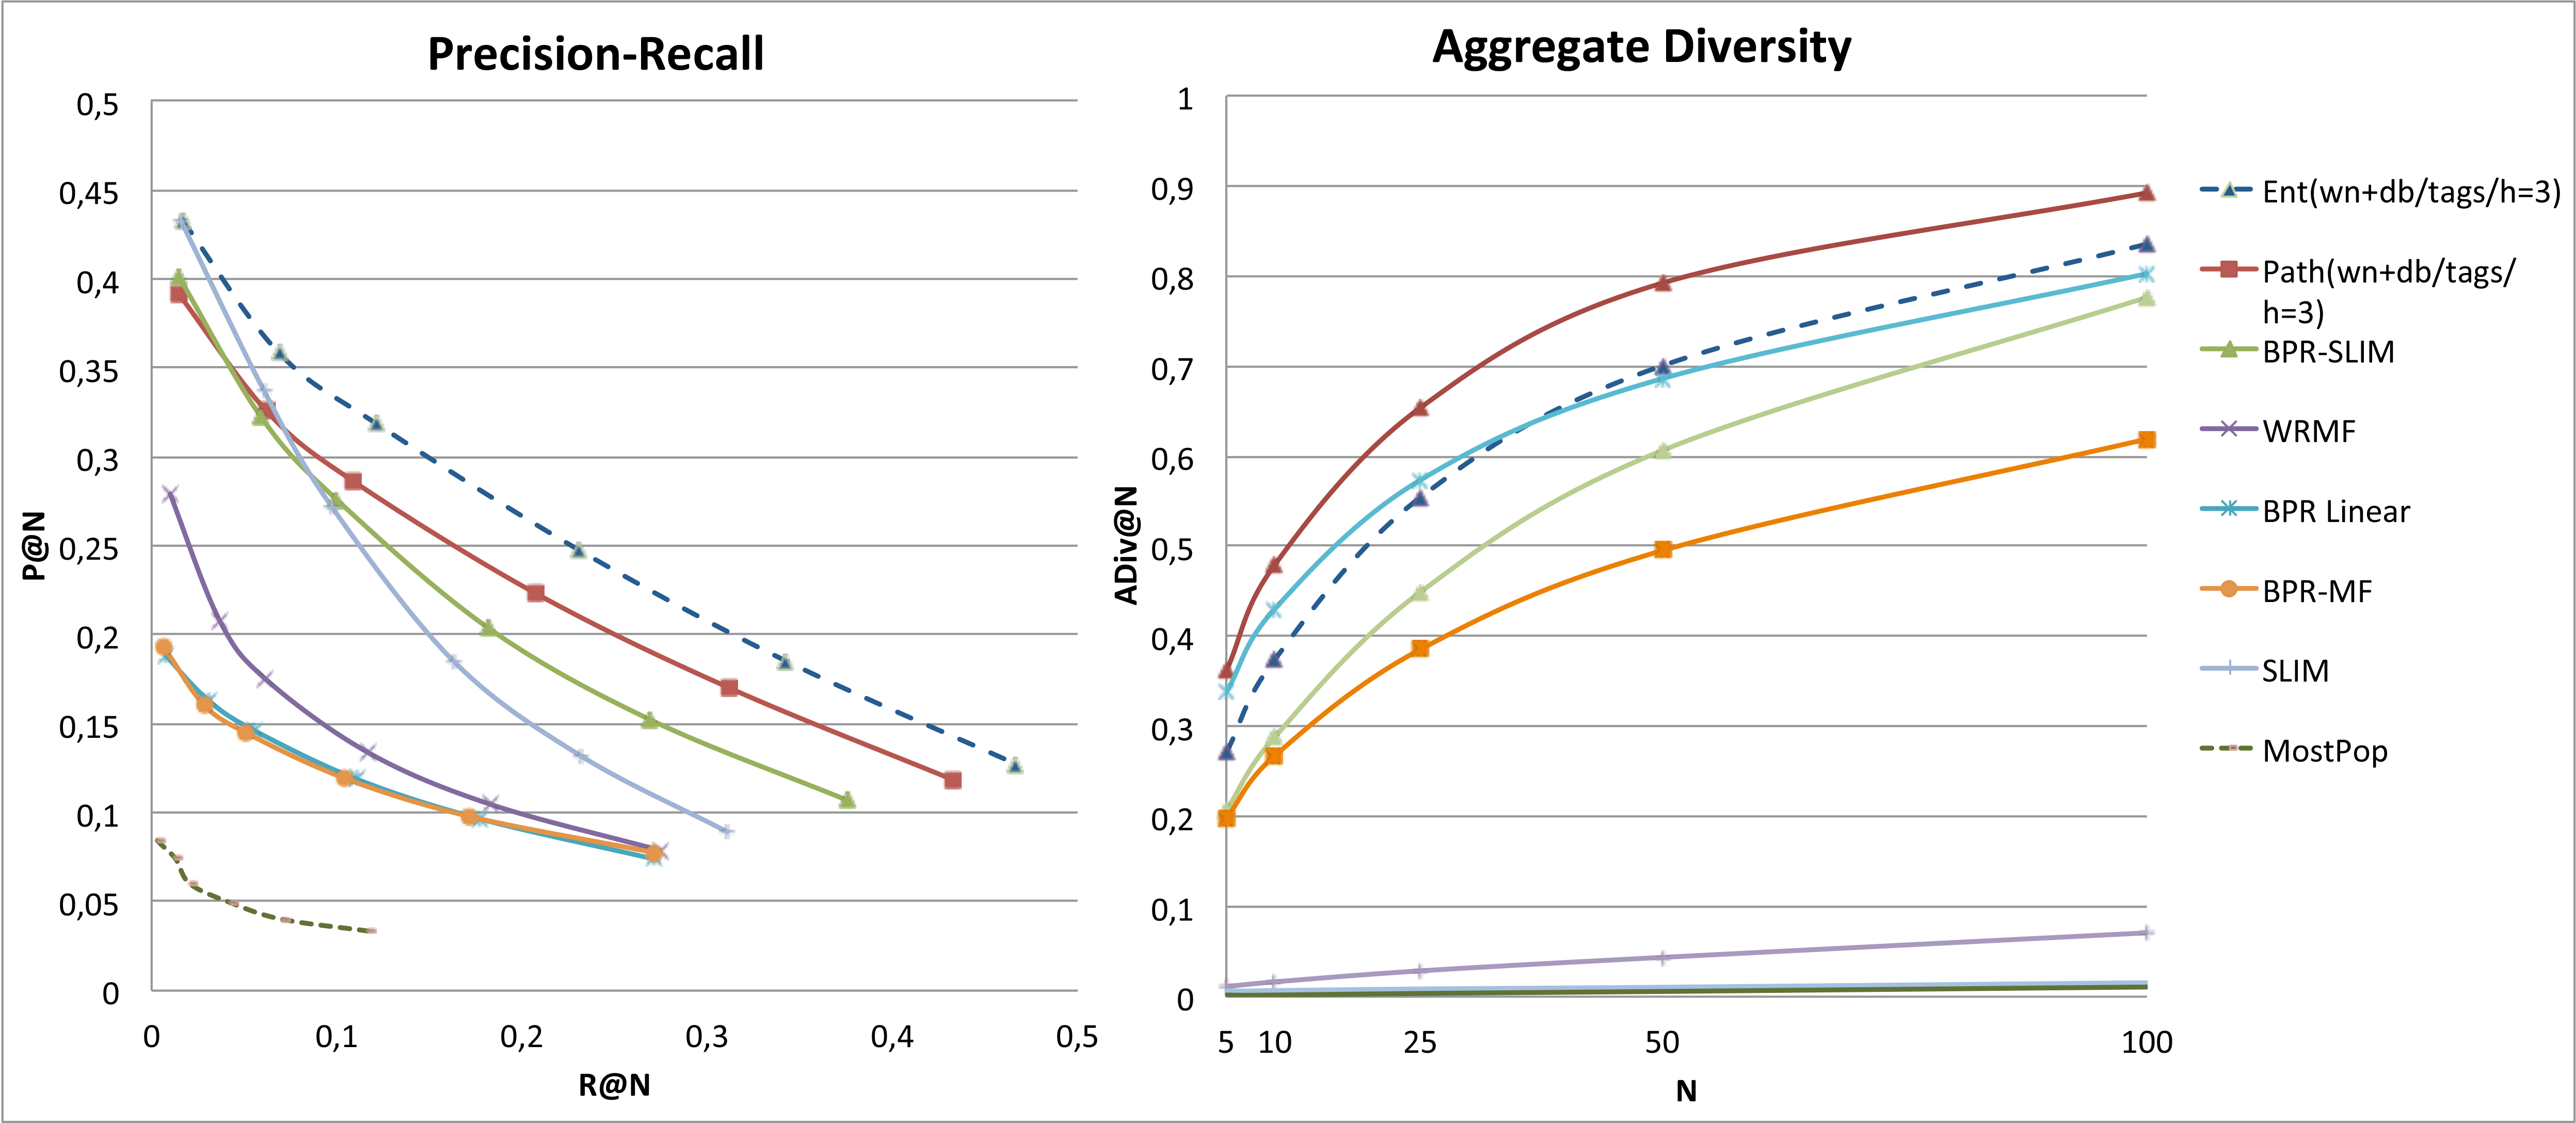
\includegraphics[width=\textwidth]{ch07_graph-rec_pics/pr_adiv_lf.png}
	\end{subfigure}
	\begin{subfigure}[b]{1\textwidth}
		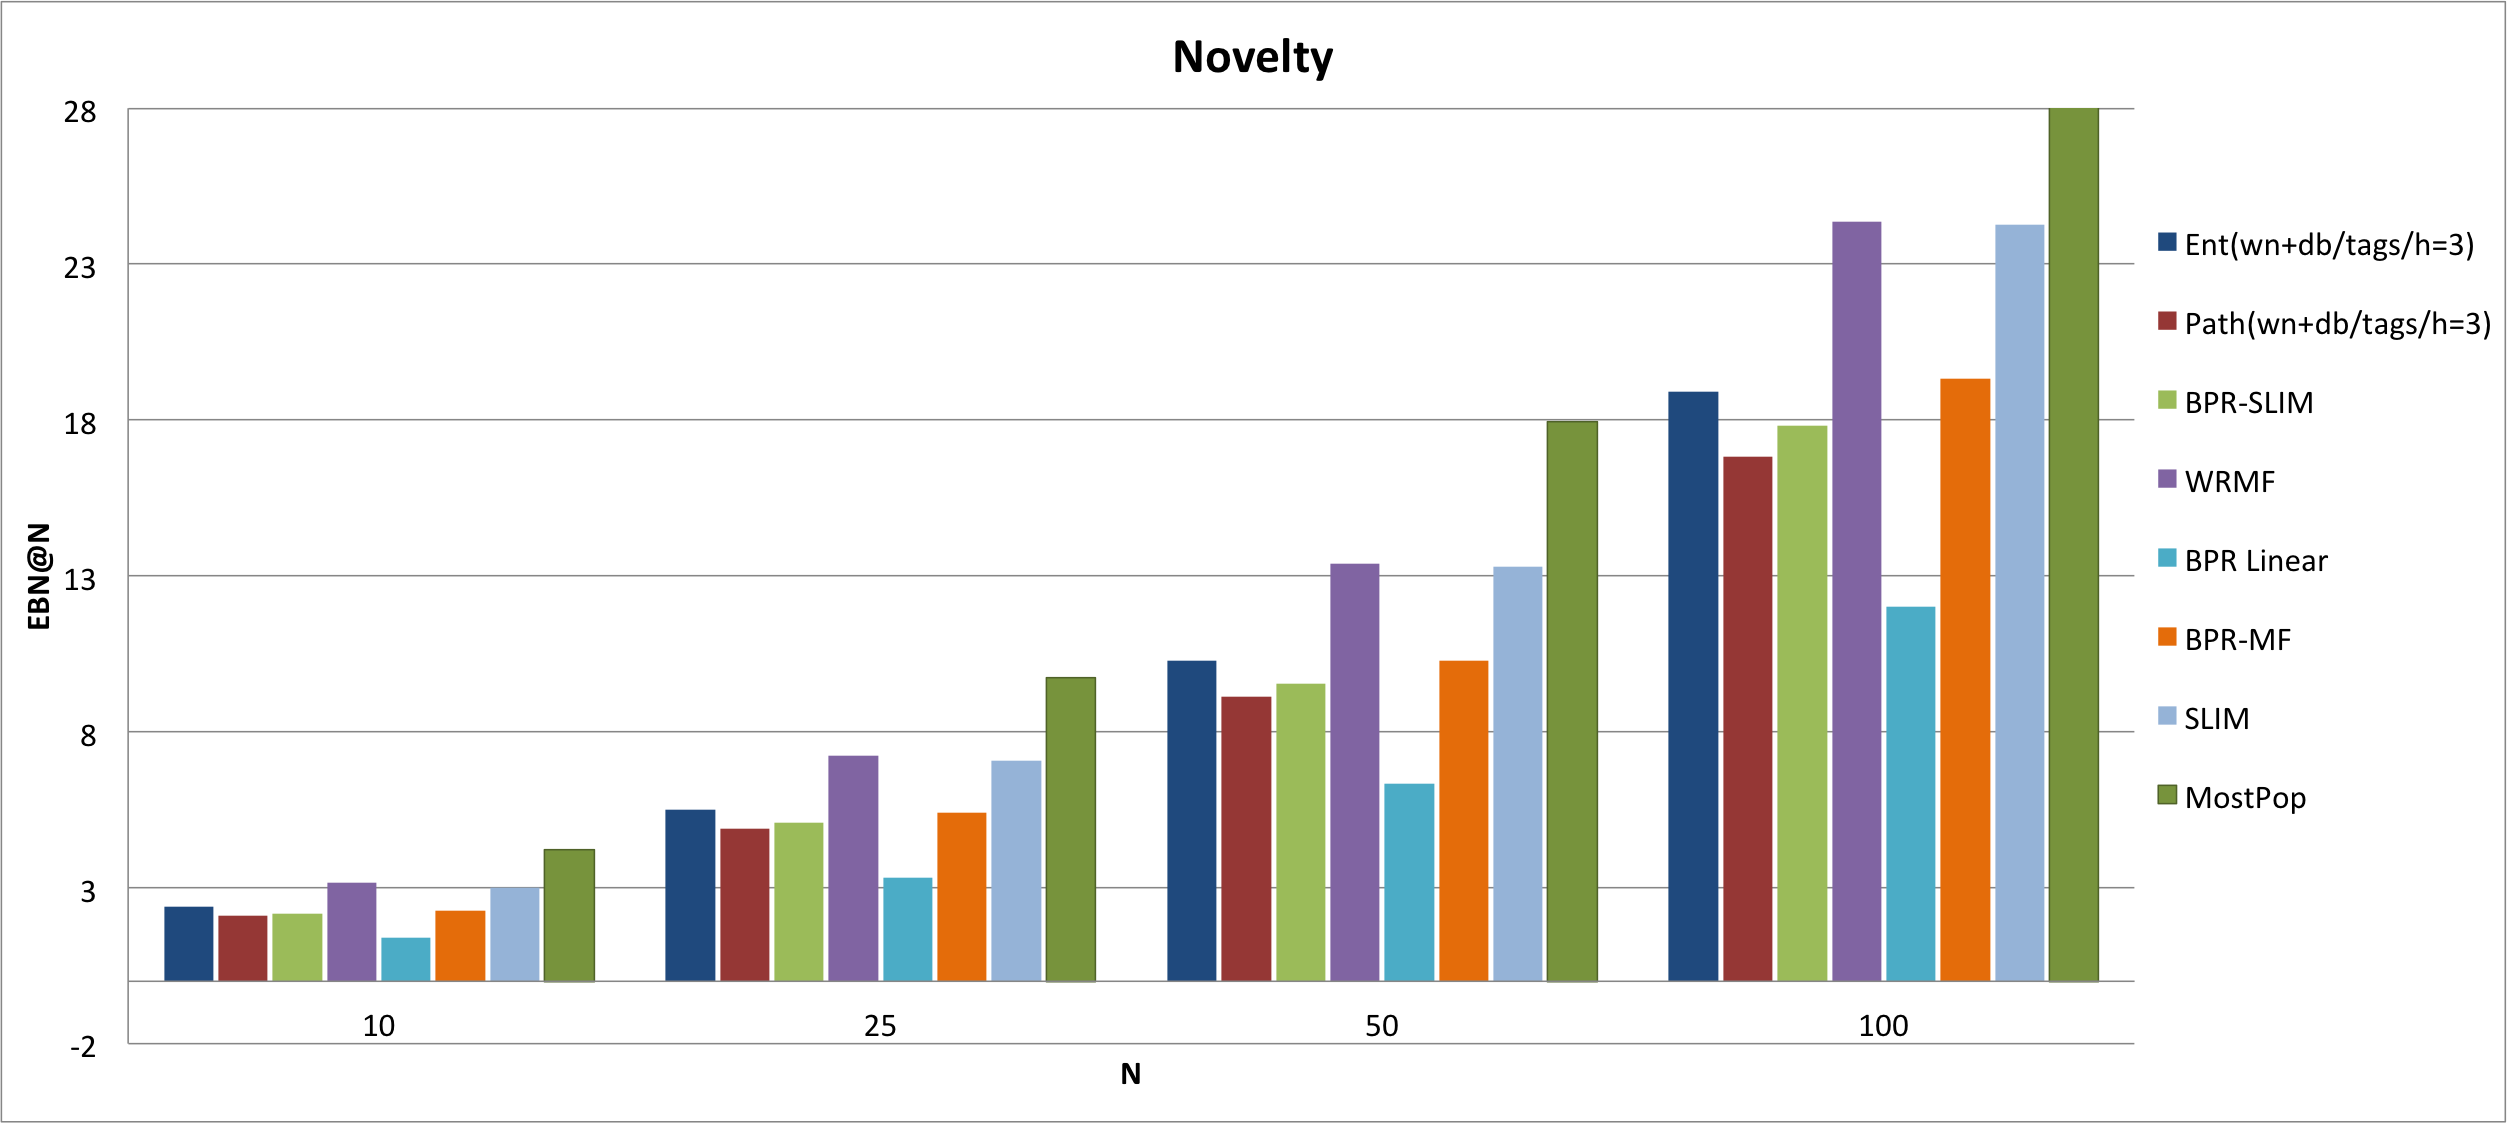
\includegraphics[width=\textwidth]{ch07_graph-rec_pics/nov_lf.png}
	\end{subfigure}
	\caption{Precision-Recall, Novelty and Aggregate Diversity plots in Last.fm dataset\label{fig:graph-rec:accur_sf}}
\end{figure*}
%%%%%%%%%%%%%%%%%%%%%%%%%%%%%%%%%%%%%%%%%%%%%%%%%%%%%%%%%%%%%%%%%%%%%%%%%%%%%%%%%%%%%

\paragraph*{\textbf{Comparison with other methods}}\label{comp}
We compared our approach with the same set of state of the art algorithms presented in the sound recommendation experiment. Based on the observations made in the previous paragraph, we used for this experiment only tags as item attribute data for \texttt{BPR Linear}.
Figure \ref{fig:graph-rec:accur_sf} shows precision-recall, novelty and aggregated diversity plots of the comparison with the other methods. We compare the competitive algorithms with the \texttt{Ent(KB/tag/h=3)} and \texttt{Path(KB/tag/h=3)} configurations which in this scenario results to be the most representative for our approach. 
Results are pretty similar to the ones observed in the sound recommendation experiment. Our two approaches largely outperforms the others in terms of accuracy. \texttt{BPR-SLIM} and \texttt{SLIM} have performance similar to our Entity-based mapping approach for low values of recommendation list length (N = 5, 10), and slightly higher that the Path-based one. %All differences between our approaches and the other methods are statistically significant ($p<0.01$) according to the paired t-test. 
Our approaches have much better novelty results than all other collaborative filtering algorithms but \texttt{BPR Linear}, which again has much lower accuracy. In terms of aggregated diversity, our approach outperforms most of the collaborative filtering algorithms. \texttt{BPR Linear} achieves similar diversity, but much lower accuracy.
Summing up, our approach is able to recommend less popular items with higher accuracy than other collaborative filtering algorithms also in this recommendation scenario. Therefore, our approach is able to improve the level of personalization of the recommended items, and  better explore the long tail also for songs recommendation.



\section{Conclusion}
\label{sec:graph-rec:conclusion}
We have presented a hybrid approach to recommend musical items, i.e. sounds and songs, by exploiting the information encoded within a knowledge graph. We conducted various experiments on two different datasets, the one of sounds coming from Freesound.org, the other one of songs gathered from Last.fm and Songfacts.com. They may be considered as representative of the two classes of users we find in the music domain: producers looking for sounds to create new music and consumers looking for new songs to listen to.

Information coming from item descriptions and tags have been %structured by means of an ontology and then further 
enriched with data coming from two external knowledge repositories: DBpedia and WordNet. Entity Linking tools have been adopted to extract relevant entities from textual sources associated to musical items, namely tags and text descriptions, thus creating a new graph encoding the knowledge associated to users, items and their mutual interactions. We then developed a recommendation engine that combines different features, that is semantic content-based ones extracted from the resulting knowledge graph and collaborative information from implicit user feedback. An evaluation with two explicit feature mappings, \textit{entity-based item neighborhood} and \textit{path-based item neighborhood}, has been conducted on both datasets in order to asses the performance of the system in terms of accuracy, diversity and novelty. 

Experimental results in sounds and songs recommendation show that the proposed approach is able to improve the quality of the recommended list with respect to state of the art collaborative filtering algorithms and with respect to other content-based baselines. Our results also show that the data related to the music knowledge domain encoded in freely available datasets such as DBpedia or WordNet have reached a quality level that makes possible its usage in the creation of recommendation engines whose target are either music producers or music consumers. The semantic enrichment of the initial knowledge graph performed by means of entity linking techniques is a good choice to boost the performances of the system in terms of novelty and aggregate diversity. A knowledge-based approach can improve the degree of personalization in the recommendations of musical items from various points of view such as prediction accuracy, catalog coverage and promote long tail recommendations. We have presented a methodology that achieves these objectives by combining semantic knowledge with collaborative information. 

Summing up, knowledge graphs can be a useful tool when properly leveraged within recommender systems for musical items. Indeed, the graph-based nature of the information they contain, on the one hand, makes possible a linkage to other graphs thus resulting in an easy plugging of new content-based data. On the other hand, by exploring the graph new connections and commonalities between items and users can be discovered and exploited while computing the recommendation list.


%\\As future chapter we are currently planning to integrate the proposed algorithm into Freesound for computing sound recommendation and perform an experimental evaluation with real users. In addition, we want to evaluate the proposed approach on different domains to generalize the results about the usage of the semantic feature expansion to improve aggregate diversity and novelty. 